\documentclass[a4paper, 12pt]{article}
%%% Работа с русским языком
\usepackage{cmap}					% поиск в PDF
\usepackage{mathtext} 				% русские буквы в формулах
\usepackage[T2A]{fontenc}			% кодировка
\usepackage[utf8]{inputenc}			% кодировка исходного текста
\usepackage[russian]{babel}	% локализация и переносы

%%% Дополнительная работа с математикой
\usepackage{amsmath,amsfonts,amssymb,amsthm,mathtools} % AMS
\usepackage{icomma} % "Умная" запятая: $0,2$ --- число, $0, 2$ --- перечисление

%% Номера формул
%\mathtoolsset{showonlyrefs=true} % Показывать номера только у тех формул, на которые есть \eqref{} в тексте.
%\usepackage{leqno} % Немуреация формул слева

%% Шрифты
\usepackage{euscript}	 % Шрифт Евклид
\usepackage{mathrsfs} % Красивый матшрифт

%%% Свои команды
\DeclareMathOperator{\sgn}{\mathop{sgn}}

%% Поля
\usepackage[left=2cm,right=2cm,top=2cm,bottom=2cm,bindingoffset=0cm]{geometry}

%% Русские списки
\usepackage{enumitem}
\makeatletter
\AddEnumerateCounter{\asbuk}{\russian@alph}{щ}
\makeatother

%%% Работа с картинками
\usepackage{graphicx}  % Для вставки рисунков
\graphicspath{{images/}{images2/}}  % папки с картинками
\setlength\fboxsep{3pt} % Отступ рамки \fbox{} от рисунка
\setlength\fboxrule{1pt} % Толщина линий рамки \fbox{}
\usepackage{wrapfig} % Обтекание рисунков и таблиц текстом

%%% Работа с таблицами
\usepackage{array,tabularx,tabulary,booktabs} % Дополнительная работа с таблицами
\usepackage{longtable}  % Длинные таблицы
\usepackage{multirow} % Слияние строк в таблице

%% Красная строка
\setlength{\parindent}{2em}

%% Интервалы
\linespread{1}
\usepackage{multirow}

%% TikZ
\usepackage{tikz}
\usetikzlibrary{graphs,graphs.standard}

%% Верхний колонтитул
% \usepackage{fancyhdr}
% \pagestyle{fancy}

%% Перенос знаков в формулах (по Львовскому)
\newcommand*{\hm}[1]{#1\nobreak\discretionary{}
	{\hbox{$\mathsurround=0pt #1$}}{}}

%% дополнения
\usepackage{float} %Добавляет возможность работы с командой [H] которая улучшает расположение на странице
\usepackage{gensymb} %Красивые градусы
\usepackage{caption} % Пакет для подписей к рисункам, в частности, для работы caption*

% подключаем hyperref (для ссылок внутри  pdf)
\usepackage[unicode, pdftex]{hyperref}

%%% Теоремы
\theoremstyle{plain}                    % Это стиль по умолчанию, его можно не переопределять.
\renewcommand\qedsymbol{$\blacksquare$} % переопределение символа завершения доказательства

\newtheorem{theorem}{Теорема}[section] % Теорема (счетчик по секиям)
\newtheorem{proposition}{Утверждение}[section] % Утверждение (счетчик по секиям)
\newtheorem{definition}{Определение}[section] % Определение (счетчик по секиям)
\newtheorem{corollary}{Следствие}[theorem] % Следстиве (счетчик по теоремам)
\newtheorem{problem}{Задача}[section] % Задача (счетчик по секиям)
\newtheorem*{remark}{Примечание} % Примечание (можно переопределить, как Замечание)
\newtheorem{lemma}{Лемма}[section] % Лемма (счетчик по секиям)

\newtheorem{example}{Пример}[section] % Пример
\newtheorem{counterexample}{Контрпример}[section] % Контрпример
\newcommand{\defeq}{\stackrel{def}{=}} % по определению
\newcommand{\defarr}{\stackrel{def}{\Rightarrow}} % следует из определения

\makeatletter
\newcommand{\eqnum}{\refstepcounter{equation}\textup{\tagform@{\theequation}}}
\makeatother % создание метки и нумерация формулы одновременно

\newcommand{\deflimk}{\lim\limits_{k\rightarrow \infty}} % лимит при k -> бесконечности
\DeclareMathOperator{\Tr}{trace} % след матрицы
\usepackage{indentfirst}


\begin{document}
    \tableofcontents{} %содержание
    \newpage


    \section{Билет 1. Основные понятия, простейшие типы дифференциальных уравнений}
\subsection{Основные понятия}

\begin{definition} 
    Уравнение вида \[F(x, y(x), y'(x), y''(x), \dots, y^{(n)}(x)) = 0\] называется обыкновенным дифференциальным уравнением,
    где $x$ -- аргумент, $y(x)$ -- неизвестная функция, $F$ -- известная непрерывная функция в области $D$.
\end{definition}

\begin{definition}
    Если это уравнение удается разрешить относительно старшей производной, такое дифференциальное
    уравнение называется разрешённым относительно старшей производной и записывается в виде
    \[y^{(n)}(x) = f(x, y(x), y'(x), y''(x), \dots, y^{(n - 1)}(x))\]
\end{definition}

Порядок уравнения определяется порядком старшей производной от $y$.

\begin{definition}
    Функция $y = \varphi(x)$ называется решением ДУ, если она $n$ раз дифференцируема и
    \[\forall x \in G \rightarrow F(x, \varphi(x), \varphi'(x), \dots, \varphi^{(n)}(x)) \equiv 0, \; (x, \varphi(x), \dots, \varphi^{(n - 1)}(x)) \in D,\]
    где $G$ -- область определения функции $\varphi(x)$ с её производными.
\end{definition}

\begin{definition}
    Система $n$ уравнений
    \begin{equation}
        \begin{cases}
            \dot x^1 = f_1(t, x^1(t), \dots, x^n(t)) \\
            \dots \\
            \dot x^n = f_n(t, x^1(t), \dots, x^n(t)) \\
        \end{cases}
    \end{equation}
    где $x^1(t), \dots, x^n(t)$ -- искомые функции, а $f_i$ -- некоторые непрерывные функции, называется нормальной системой ДУ $n$-го порядка.
\end{definition}

\begin{proposition}
    Рассмотрим ДУ $y^{(n)}(x) = f(x, y(x), y'(x), y''(x), \dots, y^{(n-1)}(x))$ $n$-ого порядка. Это уравнение эквивалентно следующей нормальной системе ДУ:
    \begin{equation}
        \begin{cases}
            \dot v_1 = v_2 \\
            \dot v_2 = v_3 \\
            \dots \\
            \dot v_{n-1} = v_n \\
            \dot v_n = f_n(x, v_1, v_2, \dots, v_n) \\
        \end{cases}
        \Leftrightarrow y^{(n)}(x) = f(x, y'(x), y''(x), \dots, y^{(n-1)}(x))
    \end{equation}
\end{proposition}

\begin{proof}
    Введём обозначения: $y = v_1(x)$, $y' = v_2(x)$,
    $y'' = v_3(x)$, $\dots$, $y^{(n - 1)} = v_n(x)$. Тогда имеем $\dot v_1 = v_2, \; \dot v_2 = v_3, \; \dots, \dot v_n = f(x, v_1, v_2, \dots, v_n)$, то есть получилась нормальная система дифференциальных уравнений $n$-ого порядка с неизвестными $v_i$.

    Обратными заменами системы уравнений можно получить исходное дифференциальное уравнение $y^{(n)}(x) = f(x, y'(x), y''(x), \dots, y^{(n-1)}(x))$.
\end{proof}

\begin{definition}
    Рассмотрим уравнение $1$-ого порядка $y' = f(x, y(x))$. Тогда задача решить это уравнение с условием $y(x_0) = y_0$ называется задачей Коши.
\end{definition}

\begin{definition}
    Пусть $\varphi(x)$ -- решение дифференциального уравнения $y' = f(x, y(x))$. График решения $\varphi(x)$ называется интегральной кривой. В силу определения функции $f(x, y)$ на множестве $\Omega$, вся интегральная кривая будет лежать в $\Omega$.
\end{definition}

\begin{definition}
    Проведём через каждую точку интегральной кривой $(x_0, y_0) \in \Omega$ малый отрезок с углом наклона по отношению к оси $x$ равным $\alpha$, причём $\tg \alpha = f'(x_0, y_0)$. Получим так называемое поле направлений. 
\end{definition}

Из построения интегральной кривой следует, что интегральная кривая в каждой своей точке касается поля направлений. Верно и обратное: кривая, касающаяся в каждой своей точке поля направлений, является интегральной кривой.

\subsection{Простейшие типы уравнений первого порядка}
\subsubsection{Уравнения в полных дифференциалах}

Рассмотрим следующее дифференциальное уравнение: $P(x, y)dx + Q(x, y)dy = 0$, причём функции $P(x, y)$ и $Q(x, y)$ непрерывны в некоторой области $D$ и $\forall (x_0, y_0) \in D \rightarrow |P(x_0, y_0)| + |Q(x_0, y_0)| > 0$. Тогда кривая 
\begin{equation}
    \gamma = 
    \begin{cases}
        x = \varphi(t) \\ 
        y = \psi(t)
    \end{cases}, \; t_1 \leqslant t \leqslant t_2
\end{equation}
называется интегральной кривой рассматриваемого уравнения, если $\forall t: t \in [t_1; t_2]$ функции $\varphi(t)$ и $\psi(t)$ непрерывно дифференцируемы, $(\varphi(t), \psi(t)) \in D$, $(\varphi_t')^2 + (\psi_t')^2 > 0$ и выполнено

\begin{equation}
    P(\varphi(t), \psi(t)) \varphi_t' + Q(\varphi(t), \psi(t)) \psi_t' = 0.
\end{equation}

\begin{definition}
    Дифференциальное уравнение $P(x, y)dx + Q(x, y)dy = 0$ называется уравнением в полных дифференциалах, если $\exists F(x, y): P(x, y)dx + Q(x, y)dy = dF(x, y)$. 
\end{definition}

Тогда $dF(x, y) = 0 \Rightarrow F(x, y) = const$, то есть $F(x, y)$ определяет неявную функцию $y(x)$.

\begin{theorem}
    Пусть функции $P(x, y)$ и $Q(x, y)$ непрерывно дифференцируемы в области $D$. Для того, чтобы уравнение $P(x, y)dx + Q(x, y)dy = 0$ являлось уравнением в полных дифференциалах, необходимо выполнение условия $\frac{\partial P}{\partial y} = \frac{\partial Q}{\partial x}$, $(x, y) \in D$. Если же область $D$ ещё и одвосвязна, то условие $\frac{\partial P}{\partial y} = \frac{\partial Q}{\partial x}$ является достаточным.
\end{theorem}

\begin{proof}
    Пусть $P(x, y)dx + Q(x, y)dy = 0$ -- уравнение в полных дифференциалах, тогда $\exists F(x, y): P(x, y)dx + Q(x, y)dy = dF(x, y) \Rightarrow P = \frac{\partial F}{\partial x}$, $Q = \frac{\partial F}{\partial y}$. По условию $P$ и $Q$ -- непрерывно дифференцируемы, тогда $\frac{\partial P}{\partial y}$ и $\frac{\partial Q}{\partial x}$ -- непрерывные функции, значит 
    \begin{equation}
        \frac{\partial P}{\partial y} = \frac{\partial^2 F}{\partial y \partial x} = \frac{\partial^2 F}{\partial x \partial y} = \frac{\partial Q}{\partial x}, \; (x, y) \in D.
    \end{equation}

    Пусть теперь $D$ -- односвязная область. Рассмотрим значение интеграла
    \[ F = \int\limits^{(x; y)}_{(x_0, y_0)} P(x, y) dx + Q(x, y) dy, \]
    который берётся по кусочно гладкой кривой $\gamma$, лежащей в $D$ и соединяющей точки $(x_0, y_0)$ и $(x; y)$. Пусть $\frac{\partial P}{\partial y} = \frac{\partial Q}{\partial x}$. Тогда по теореме о независимости интеграла от пути интегрирования выходит, что значение интеграла не зависит от пути интегрирования $\gamma$, а является функцией от $(x, y)$, значит $F = F(x, y)$ -- функция и $P(x, y)dx + Q(x, y)dy = dF(x, y)$.
\end{proof}

\begin{definition}
    Непрерывно дифференцируемая функция $\mu(x, y) \neq 0$ в области $G$ называется интегрирующим множителем для уравнения $P(x, y) dx + Q(x, y) dy = 0$, если уравнение $\mu(x, y) (P(x, y) dx + Q(x, y) dy) = 0$ -- уравнение в полных дифференциалах, а исходное уравнение $P(x, y) dx + Q(x, y) dy = 0$ не является уравнением в полных дифференциалах.
\end{definition}

Если $\mu(x, y)$ -- интегрирующий множитель, то для достаточного условия имеем (с учётом требований теоремы выше)
\[ \frac{\partial (\mu P)}{\partial y} = \frac{\partial (\mu Q)}{\partial x} \Leftrightarrow P \frac{\partial \mu}{\partial y} + \mu \frac{\partial P}{\partial y} = Q \frac{\partial \mu}{\partial x} + \mu \frac{\partial Q}{\partial x}. \]

Полученное уравнение не легче исходного, так как теперь задача свелась к нахождению $\mu$. Обычно интегрирующий множитель ищут в виде $\mu(x), \; \mu(y), \; \mu(x^2 + y^2), \; \mu (x^{\alpha}, y^ {\beta})$.

\subsubsection{Уравнения с разделяющимися переменными}

Рассмотрим ДУ вида $P(y)dx + Q(x)dy = 0$, где $P(y) \in C_{[y_1; y_2]}^1$, $Q(x) \in C_{[x_1; x_2]}^1$. Если $\exists y_0: P(y_0) = 0$ или  $\exists x_0: Q(x_0) = 0$, тогда
\begin{equation}
    \begin{cases}
        x = t \\ 
        y = y_0
    \end{cases} \;
    \text{или} \;
    \begin{cases}
        x = x_0 \\ 
        y = t
    \end{cases}
\end{equation}
являются интегральными кривыми рассматриваемого ДУ соответственно. Если же выполняется $P(y) \neq 0$ и $Q(x) \neq 0$, то применим к уравнению интегрирующий множитель
\[ \mu(x, y) = \frac{1}{P(y)Q(x)}, \]
получив уравнение в полных дифференциалах
\begin{equation}
    \frac{dx}{Q(x)} + \frac{dy}{P(y)} = 0.
\end{equation}

Значение $\mu(x, y)$ действительно является интегрирующим множителем, так как выполняется
\begin{equation}
    \frac{\partial}{\partial y} \left( \frac{1}{Q(x)} \right) =  \frac{\partial}{\partial x} \left( \frac{1}{P(y)} \right) = 0.
\end{equation}

Тогда
\begin{equation}
    dF(x, y) = \frac{dx}{Q(x)} + \frac{dy}{P(y)} \Rightarrow \frac{\partial F}{\partial x} = \frac{1}{Q(x)} \Rightarrow F(x, y) = \int\limits_{x_0}^{x} \frac{dt}{Q(t)} + C(y),
\end{equation}

\begin{equation}
    \frac{\partial F}{\partial y} = \frac{1}{P(y)} = C'(y) \Rightarrow C(y) = \int\limits_{y_0}^{y} \frac{dt}{P(t)} \Rightarrow F(x, y) = \int\limits_{x_0}^{x} \frac{dt}{Q(t)} + \int\limits_{y_0}^{y} \frac{dt}{P(t)} = const.
\end{equation}

Точка $(x_0, y_0)$ -- произвольная точка в области определения функций $P$ и $Q$.

\begin{definition}
    Если дифференциальное уравнение вида $P_1(x, y)dx + Q_1(x, y)dy = 0$ может быть сведено к виду $P(y)dx + Q(x)dy = 0$, то такое уравнение называется уравнением с разделяющимися переменными.
\end{definition}

\begin{proposition}
    Задача Коши уравнения с разделяющимися переменными $P(y)dx + Q(x)dy = 0$ задаётся в виде $y(x_1) = y_1$, а её решение в виде 
    \begin{equation}
        \int\limits_{x_1}^{x} \frac{dt}{Q(t)} + \int\limits_{y_1}^{y} \frac{dt}{P(t)} = 0.
    \end{equation}
\end{proposition}

\subsubsection{Однородные уравнения}

Рассмотрим дифференциальное уравнение вида
\[ y' = g \left( \frac{y}{x} \right), \]
которое назовём уравнением с однородной правой частью, где $g(z)$ -- непрерывная функция на некотором промежутке. Сделаем замену $v(x) = \frac{y}{x}$, тогда $y(x) = v(x) \cdot x$, $y_x' = x \cdot v_x' + v = g(v)$, откуда имеем $x \frac{dv}{dx} = g(v) - v$. Если $\exists v_0: g(v_0) = v_0$, то $v_0$ -- решение уравнения $x \frac{dv}{dx} = g(v) - v$. Если же $v \neq g(v)$, тогда
\begin{equation}
    \frac{dv}{g(v) - v} = \frac{dx}{x} \Rightarrow \ln |x| + C = \int\limits_{v_0}^{v} \frac{dt}{g(t) - t}.
\end{equation}

Таким образом, найдено решение исходного уравнения с однородной правой частью в квадратурах.

\begin{definition}
    Функция $F(x^1, x^2, \dots, x^n)$ называется однородной степени $m$, если $\forall \lambda > 0 \longrightarrow F(\lambda x^1, \lambda x^2, \dots,  \lambda x^n) = \lambda^m F(x^1, x^2, \dots, x^n)$.
\end{definition}

\begin{example}
    Рассмотрим уравнение $P(x, y) dx = Q(x, y) dy$. Если $P(x, y)$ и $Q(x, y)$ -- однородные функции степени $m$, тогда
    \begin{equation}
        \frac{dy}{dx} = \frac{P(x, y)}{Q(x, y)} = \frac{x^m P(1, \frac{y}{x})}{x^m Q(1, \frac{y}{x})} = \frac{P(1, \frac{y}{x})}{Q(1, \frac{y}{x})} = g \left( \frac{y}{x} \right)
    \end{equation}
    Таким образом исходное уравнение свелось к уравнению с однородной правой частью.
\end{example}

\subsubsection{Линейные уравнения первого порядка}

\begin{definition}
    Дифференциальное уравнение вида $y' + a(x) y = f(x)$ -- линейное дифференциальное уравнение первого порядка. Дифференциальное уравнение вида $y' + a(x) y = 0$ -- линейное однородное дифференциальное уравнение первого порядка. При этом $a(x) \in C_{I(x)}$, $f(x) \in C_{I(x)}$, где $I(x)$ -- область, на которой определены функции $a(x)$ и $f(x)$. 
\end{definition}

Введём оператор $L = \frac{d}{dx} + a(x)$, который действует на множество непрерывно дифференцируемых функций $\varphi \in C^1_{I(x)}$. Тогда уравнение $y' + a(x) y = f(x)$ переписывается в виде $L(y) = f(x)$, а уравнение $y' + a(x) y = 0$ переписывается в виде $L(y) = 0$.

\begin{theorem}
    Введённые оператор $L = \frac{d}{dx} + a(x)$ -- линейный оператор.
\end{theorem}

\begin{proof}
    Рассмотрим линейную комбинацию $c_1 \varphi_1(x) + c_2 \varphi_2(x)$:
    \begin{equation}
        L(c_1 \varphi_1(x) + c_2 \varphi_2(x)) = (c_1 \varphi_1 + c_2 \varphi_2)' + a(x) (c_1 \varphi_1 + c_2 \varphi_2) = c_1 L(\varphi_1) + c_2 L(\varphi_2)
    \end{equation}
    Таким образом, $L(c_1 \varphi_1 + c_2 \varphi_2) = c_1 L(\varphi_1) + c_2 L(\varphi_2)$, то есть $L$ -- линейный оператор.
\end{proof}

\begin{proposition}
    Решением уравнения $y' + a(x) y = 0$ является
    \begin{equation}
        y = C e^{-\int\limits_{x_0}^{x} a(t) dt}, \; C \in \mathbb{R}.
    \end{equation}
\end{proposition}

\begin{proof}
    Найдём решение уравнения $y' + a(x) y = 0$: 
    \begin{equation}
        \frac{dy}{y} = -a(x) dx \Rightarrow \ln |y| = - \int\limits_{x_0}^{x} a(t) dt + \ln C \Rightarrow |y| = C e^{-\int\limits_{x_0}^{x} a(t) dt}, \; C > 0
    \end{equation}
    Раскрывая модуль и объединяя полученное решение с нулевым ($y \equiv 0$), имеем
    \begin{equation}
        y = C e^{-\int\limits_{x_0}^{x} a(t) dt}, \; C \in \mathbb{R}.
    \end{equation}
\end{proof}

\begin{proposition}
    Решением уравнения $y' + a(x) y = f(x)$ является
    \begin{equation}
        y = C_0 e^{-\int\limits_{x_0}^{x} a(t) dt} + \int\limits_{x_0}^{x} f(t) e^{- \int\limits_{t}^{x} a(s) ds} dt, \; C_0 \in \mathbb{R}.
    \end{equation}
\end{proposition}

\begin{proof}
    Найдём решение уравнения $y' + a(x) y = f(x)$: воспользуемся уже найденным решением однородного уравнения, применяя метод вариации постоянной. То есть будем искать решение в виде
    \begin{equation}
        y = C(x) e^{-\int\limits_{x_0}^{x} a(t) dt}.
    \end{equation}
    Подставим это решение в исходное уравнение:
    \begin{equation}
        C'(x) e^{-\int\limits_{x_0}^{x} a(t) dt} - a(x) C(x) e^{-\int\limits_{x_0}^{x} a(t) dt} + a(x) C(x) e^{-\int\limits_{x_0}^{x} a(t) dt} = f(x)
    \end{equation}
    \begin{equation}
        C'(x) e^{-\int\limits_{x_0}^{x} a(t) dt} = f(x) \Rightarrow C(x) = \int\limits_{x_0}^{x} f(t) e^{\; \int\limits_{x_0}^{t} a(s) ds} dt + C_0 
    \end{equation}
    Таким образом найден вид $C(x)$. Теперь подставим эту функцию:
    \begin{equation}
        y = C_0 e^{-\int\limits_{x_0}^{x} a(t) dt} + e^{-\int\limits_{x_0}^{x} a(t) dt} \int\limits_{x_0}^{x} f(t) e^{\; \int\limits_{x_0}^{t} a(s) ds} dt
    \end{equation}
    \begin{equation}
        y = C_0 e^{-\int\limits_{x_0}^{x} a(t) dt} + \int\limits_{x_0}^{x} f(t) e^{- \int\limits_{t}^{x} a(s) ds} dt
    \end{equation}
    
    Из полученного решения видно, что оно является суммой решения однородного уравнения и частного решения. 
\end{proof}

\begin{proposition}
    Если $\varphi_1(x)$ и $\varphi_2(x)$ -- некоторые решения уравнения $y' + a(x) y = f(x)$, то $z(x) = \varphi_1(x) - \varphi_2(x)$ -- решение однородного уравнения $y' + a(x) y = 0$.
\end{proposition}

\begin{proof}
    По условию $\varphi_1' + a(x) \varphi_1 = f(x)$, $\varphi_2' + a(x) \varphi_2 = f(x)$, откуда очевидно, что $(\varphi_1 - \varphi_2)' + a (\varphi_1 - \varphi_2) = 0$. Обозначив $z = \varphi_1 - \varphi_2$, получим $z' + a(x) z = 0$, то есть $z$ -- решение однородного уравнения.
\end{proof}

    \subsection{Уравнения Бернулли и Риккати}
\subsubsection{Уравнение Бернулли}

\begin{definition}
	ДУ вида $ \boxed{y' + a(x)\cdot y = y^r \cdot f(x)}^{\eqnum\label{eq:Ber}} $, где $a(x), f(x)$ -- непрерывные функции на $(\alpha, \beta)$, $r \in \mathbb{ R }, r \neq 1$ называется уравнением Бернулли. \\
\end{definition}

\begin{proposition} %% тут бы добавить расширение для переноса символов на новую строку, чтобы не приходилось дублировать стрелку 
	Если $ r > 0 $, то $ y \equiv 0 $ - тривиальное решение. Пусть $ y \neq 0$, разделим ДУ на $ y^r \Rightarrow \frac{ y' }{ y^r } + a(x) \cdot y^{ 1-r } = f(x).$ Замена: $ u(x) = y^{ 1-r } \Rightarrow u' = ( 1-r ) \cdot y^{ -r } \cdot y' \Rightarrow$ \\ $\Rightarrow \underbracket{ \frac{ 1 }{ 1-r } \cdot u' + a(x)\cdot u = f(x) }$ -- свелось к линейному уравнению. 
\end{proposition}

\subsubsection{Уравнение Риккати}

\begin{definition}
	ДУ вида $ \boxed{y' + a(x) \cdot y^2 + b(x) \cdot y = c(x)}^{\eqnum\label{eq:Ric}} $, где $a(x), b(x), c(x)$ -- непрерывные функции на $(\alpha, \beta)$, называется уравнением Риккати. 
\end{definition}

\begin{proposition}	
	В общем случае уравнение Риккати не допускает решений в квадратурах, однако, если известно некоторое решение $ y = \varphi (x) $, то сделав замену $ y = u + \varphi $, получаем: $ \varphi' + a \varphi^2 + b\varphi = c $ \\ $ \varphi' + u' + a \varphi^2 + 2 a\varphi u + au^2 + b\varphi + bu = c \Rightarrow u' = - au^2 - (2a\varphi + b)u $ -- свелось к уравнению Бернулли.
\end{proposition}

\subsection{Методы понижения порядка дифференциальных уравнений}
\begin{proposition}

	Рассмотрим множество преобразований плоскости \\ $ \boxed{\bar{x} = \varphi(x, y, \lambda), \bar{y} = \psi (x, y, \lambda)}^{\eqnum\label{eq:trans}} $. В \eqref{eq:trans} каждому $ \lambda \in \mathcal{ D }  \subset \mathbb{ R } $ соответствует некоторое преобразование, например, $ \bar{x} = \lambda x, \bar{y} = \lambda y, \lambda > 0 $ -- гомотетия. Множество преобразований \eqref{eq:trans}  является группой преобразований, если оно содержит любую композицию \eqref{eq:trans}, т.е. 
	\[ \forall \lambda_1, \lambda_2 \, \exists \lambda_0 : \forall x, y \rightarrow \varphi(\varphi(x, y, \lambda_1), \psi(x, y, \lambda_1), \lambda_2) = \varphi(x, y, \lambda_0),\]
	\[ \psi(\varphi(x, y, \lambda_1), \psi(x, y, \lambda_1), \lambda_2) = \psi(x, y, \lambda_0),\]
	если содержит тождественное преобразование, т.е. 
	\[ \exists \lambda_0: \forall x, y \rightarrow \varphi(x, y, \lambda_0) = x; \ \psi(x, y, \lambda_0) = y,\]
	и если вместе с любым преобразованием содержит и обратное: 
	\[ \forall \lambda \in \mathcal{D} \colon \exists \lambda_0 \colon x = \overline{\varphi}  (\bar{x}, \bar{y}, \lambda_0); \ y = \overline{\psi} (\bar{x}, \bar{y}, \lambda_0) \]
	Таким образом, если \eqref{eq:trans} -- группа, то $ x = \overline{\varphi} (\bar{x}, \bar{y}, \lambda), \ y = \overline{\psi}  (\bar{x}, \bar{y}, \lambda);$ если в ДУ $ y' = f(x, y)$ осуществить переход к новым координатам, то \\
	$$
	\frac{dy}{dx} = \frac{ \overline{\psi}'_{ \bar{x} } d\bar{x} +  \overline{\psi}'_{ \bar{y} } d\bar{y} }{ \overline{\varphi}'_{\bar{x}} d\bar{x} + \overline{\varphi}'_{\bar{y}} d\bar{y}} = f(\overline{ \varphi }(\bar{x}, \bar{y}, \lambda), \overline{ \psi }(\bar{x}, \bar{y}, \lambda)) = \tilde{f}(\bar{x}, \bar{y}, \lambda) \Rightarrow
	$$	
	\begin{equation} \label{eq:def}
	\Rightarrow \frac{ \overline{\psi}'_{ \bar{x} } + \overline{\psi}'_{ \bar{y} } \cdot \frac{d\bar{y}}{d\bar{x}} }{ \overline{\varphi}'_{\bar{x}} + \overline{\varphi}'_{\bar{y}} \cdot \frac{d\bar{y}}{d\bar{x}} } = \tilde{f}(\bar{x}, \bar{y}, \lambda) \Rightarrow \frac{d\bar{y}}{d\bar{x}} = \frac{\tilde{f} \cdot  \overline{\varphi}'_{\bar{x}} - \overline{\psi}'_{\bar{x} } }{ \overline{\psi}'_{\bar{y}} - \tilde{f} \cdot \overline{\varphi}'_{\bar{y}}}
	\end{equation}  
	
	\eqref{eq:def} является записью $ y' = f(x, y) $ в новых координатах. Говорят, что $ y' = f(x, y) $ допускает группу $ x = \overline{\varphi} (\bar{x}, \bar{y}, \lambda), \ y =  \overline{\psi} (\bar{x}, \bar{y}, \lambda)$, если оно не изменяется при переходе к новым переменным, т.е. $ \frac{d\bar{y}}{d\bar{x}} = f(\bar{x}, \bar{y}) $.
\end{proposition}

\begin{corollary}
	Рассматриваем уравнения вида $ \boxed{F(x, y, y', y'') = 0}^{\eqnum\label{eq:F0}} $. \\
	\begin{enumerate}
		\item $\boxed{F(x, y', y'') = 0}^{\eqnum\label{eq:F1}}$ Замена $y'(x) = v(x) \Rightarrow y''(x) = v'(x) \ \text{и } \eqref{eq:F1}$ в этом случае имеет вид $ F(x, v(x), 	v'(x)) = 0 \xrightarrow[\text{решаем}]		{} v(x) = g(x, C_1)$. Тогда решение $\eqref{eq:F1}$ запишется в виде $ \frac{dy}{dx} = g(x, C_1) \Rightarrow y(x) = C_2 + \int g(x, C_1)dx$. Заметим, что $ \eqref{eq:F1} $ допускает группу сдвига $ x = \bar		{x}, \  y = \bar{y} + y_0 $.
		\item $\boxed{F(y, y', y'') = 0}^{\eqnum\label{eq:F2}} \ (\text{не содержит явно x}) $.  Замена: $ y' = v(y),$ тогда \\
			$y'' = \frac{dv}{dx} = \frac{dv}{dy}\frac{dy}{dx} = v\frac{dv}{dy} \Rightarrow F(y, v, v\frac{dv}{dy}) = 0$ -- ДУ первого порядка. \\
			Решение $ v(y) = g(y, C_1) \Rightarrow  \frac{dy}{dx} = g(y, C_1) \Rightarrow $ Решение $\eqref{eq:F2}$: $ \int \frac{dy}{g(y, C_1)} = x + C_2. $ \\
			Заметим, что $ \eqref{eq:F2} $ допускает группу сдвига $ x = \bar{x} + x_0 $, $ y = \bar{y} $.
		\item $ \boxed{F(x, y, y', y'') = 0 \  \text{и} \ F - \text{однородная функция степени m по } y, y', y''}$, т.е. $ \forall \lambda > 0 \rightarrow$ \\
			$F(x, \lambda y, \lambda y', \lambda y'') = \lambda^m \cdot F(x, y, y', y'') $. В таком случае ДУ допускает группу \\ 
			$ x = \bar{x}, y = \lambda \bar{y}$. \\
			Замена: $z(x) = \frac{y'}{y} \Rightarrow y' = z(x)y \Rightarrow y'' = z'  y + zy' = z'y + z^{2}y = y \cdot (z' + z^2) \Rightarrow F(x, y, zy, y(z' + z^2)) = 0 \Rightarrow y^m \cdot F(x, 1, z, z' + z^2) = 0
			$ -- относительно z имеем уравнение первого порядка. \\
			Если его решение $z(x) = g(x, C_1),$ то $\frac{y'}{y} = g(x, C_1) \Rightarrow \frac{dy}{y} = g(x, C_1)dx \Rightarrow$ \\ 
			$ \ln|y| = \int g(x, C_1)dx + C_2 $.
		\item[4*.] Будем говорить, что функция $ F(x, y, y', y'', ..., y^{(n)})$ является квазиоднородной функцией степени $ r $, если $ \exists \alpha \in \mathbb{ R }: 			\forall \lambda > 0: F(\lambda x, 			\lambda^{\alpha}y, \lambda^{\alpha - 1}y', ..., \lambda^{\alpha - n}y^{(n)} ) =$ \\ $ = \lambda^r \cdot F(x, y, ..., y^{(n)}). $ \\
			Рассмотрим группу преобразований:
			\begin{equation} \label{eq:conv}
				\left\{
				\begin{aligned} 
				x &= \lambda \bar{x}  \\
				y &= \lambda^{\alpha} \bar{y}\\   
				\end{aligned}
				\right.\text{,}  \quad  \text{где } \lambda > 0                                            
			\end{equation}

			Такую группу преобразований перепишем в виде: 
			\[
				\left\{
				\begin{aligned}
					x &= e^{\beta} \cdot \bar{x}  \\
					y &= e^{\alpha \beta} \bar{y} \\   
				\end{aligned}
				\right.                                                          
			\]
			Если функция $F$ является квазиоднородной, то $\eqref{eq:F0}$ допускает группу растяжений $\eqref{eq:conv}$: \\
			\[
				\boxed{F(x, y, y', y'') = 0} \xrightarrow[\text{преобр.}]{} F(\lambda \bar{x}, \lambda^{\alpha} \bar{y}, \lambda^{\alpha - 1} \bar{y}', \lambda^{\alpha - 2} \bar{y}'') = \lambda^{r} \cdot F(\bar{x}, \bar{y}, \bar{y}', \bar{y}'') = 0
			\]
			\[
				\Downarrow
			\]
			\[
				F(\bar{x}, \bar{y}, \bar{y}', \bar{y}'') = 0
			\]
			\ \\
			\[
			\text{Замена: }\left\{
			\begin{aligned}
				x &= e^{t}  \\
				y &= z(t) \cdot e^{\alpha t}\\   
			\end{aligned}
			\right. \quad
			\Rightarrow  \quad y'_x = \frac{y'_t}{x'_t} = \frac{z'_t \cdot e^{\alpha t} +  z \cdot \alpha \cdot e^{\alpha t}}{e^t} =  e^{(\alpha  -  1)t} \cdot (z'_t  + \alpha z)                                              
			\]
			\[
			\Downarrow
			\]
			\[
				y''_{xx} = \frac{(y'_x)'_t}{x'_t} = \frac{(\alpha - 1) \cdot e^{(\alpha - 1)t} \cdot (z'_t + \alpha z) + e^{(\alpha - 1)t} \cdot (z''_{tt} + \alpha z'_t)}{e^t} = 
			\]	
			\[	
				= e^{(\alpha - 2)t} \cdot (z''_{tt} + (2\alpha - 1)\cdot z'_t + \alpha \cdot (\alpha - 1)z)
			\]
			\[
			\Downarrow
			\]
			\[
				F(e^t, z \cdot e^{\alpha t}, e^{(\alpha - 1)t} \cdot (z'_t + \alpha z), e^{(\alpha - 2)t}(z''_{tt} + (2\alpha - 1)z'_t + \alpha \cdot (\alpha - 1)z) ) =
			\]
			\[
				= e^{rt} \cdot F(1, z, z'_t + \alpha z, z''_{tt} + (2\alpha - 1)z'_t + \alpha \cdot (\alpha - 1)z) = 0 \; -
			\]
			не содержит $t$, т.е. свелось к случаю 2 и можно понизить порядок уравнения.
	\end{enumerate}
\end{corollary}

\subsection{Метод введения параметра для уравнения первого порядка, не разрешенного относительно производной}
\begin{proposition}
	Рассмотрим $ \boxed{F(x,  y, y') = 0}^{\eqnum\label{eq:F4}} \ $, где $ F(x, y, y') $ как функция трёх переменных является непрерывно дифференцируемой в области $ D \subset \mathbb{ R }^3 $. \\
	Решение уравнения $F(x, y, y') = 0 $ будем представлять как кривую в параметрическом виде: \\
	\begin{equation} \label{eq:int}
	\gamma: \	\left\{
	\begin{aligned}
		x &= \varphi(t)  \\
		y &= \psi(t) \\   
	\end{aligned}
	\right. \ t \in [t_1, t_2], \ \varphi(t), \psi(t) \in C^1_{[t_1, t_2]}                                             
	\end{equation}
	Кривая \eqref{eq:int} является интегральной кривой \eqref{eq:F4} $ \Rightarrow $ \\
	\begin{equation} \label{eq:F5}
	 \Rightarrow F\left(\varphi(t), \psi(t), \frac{\psi'_t}{\varphi'_t}\right) = 0 \ \ \forall t \in [t_1, t_2] 
	\end{equation}
	Будем решать эквивалентную систему положив $p = \frac{dy}{dx} $: 
	\begin{equation} \label{eq:Fs}
		\left\{
		\begin{aligned}
			&F(x, y, p) = 0  \\
			&dy = pdx \\   
		\end{aligned}
		\right.                                                          
	\end{equation}
\end{proposition}

\begin{proposition}
	Уравнение \eqref{eq:F4} эквивалентно системе \eqref{eq:Fs}.
\end{proposition}

\begin{proof}
	Пусть $\gamma $ -- интегр. кривая \eqref{eq:int}. Положим $ p = \frac{\psi'}{\varphi'} = \frac{dy}{dx} $ -- второе уравнение в системе \eqref{eq:Fs} выполнено, а первое выполнено в силу подстановки в \eqref{eq:F5}. Обратно, пусть $x(t) = \varphi(t), \ y(t) = \psi(t), \; p$ -- решение \eqref{eq:F5}. Из второго уравнения системы
	$ p = \frac{\psi'_t}{\varphi'_t}$, подставляем в первое уравнение системы и получаем само уравнение \eqref{eq:F5}.\\
\end{proof}

\begin{proposition}
	Рассмотрим метод решения \eqref{eq:F4}, который называется методом введения параметра. \\
	Первое уравнение в системе \eqref{eq:Fs} рассмотрим как задающее в $\mathbb{ R }^3_{(x, y, p)} $ гладкую поверхность $S$, для которой параметрическое представление имеет вид:
	\begin{figure}[!h]
		\centering
		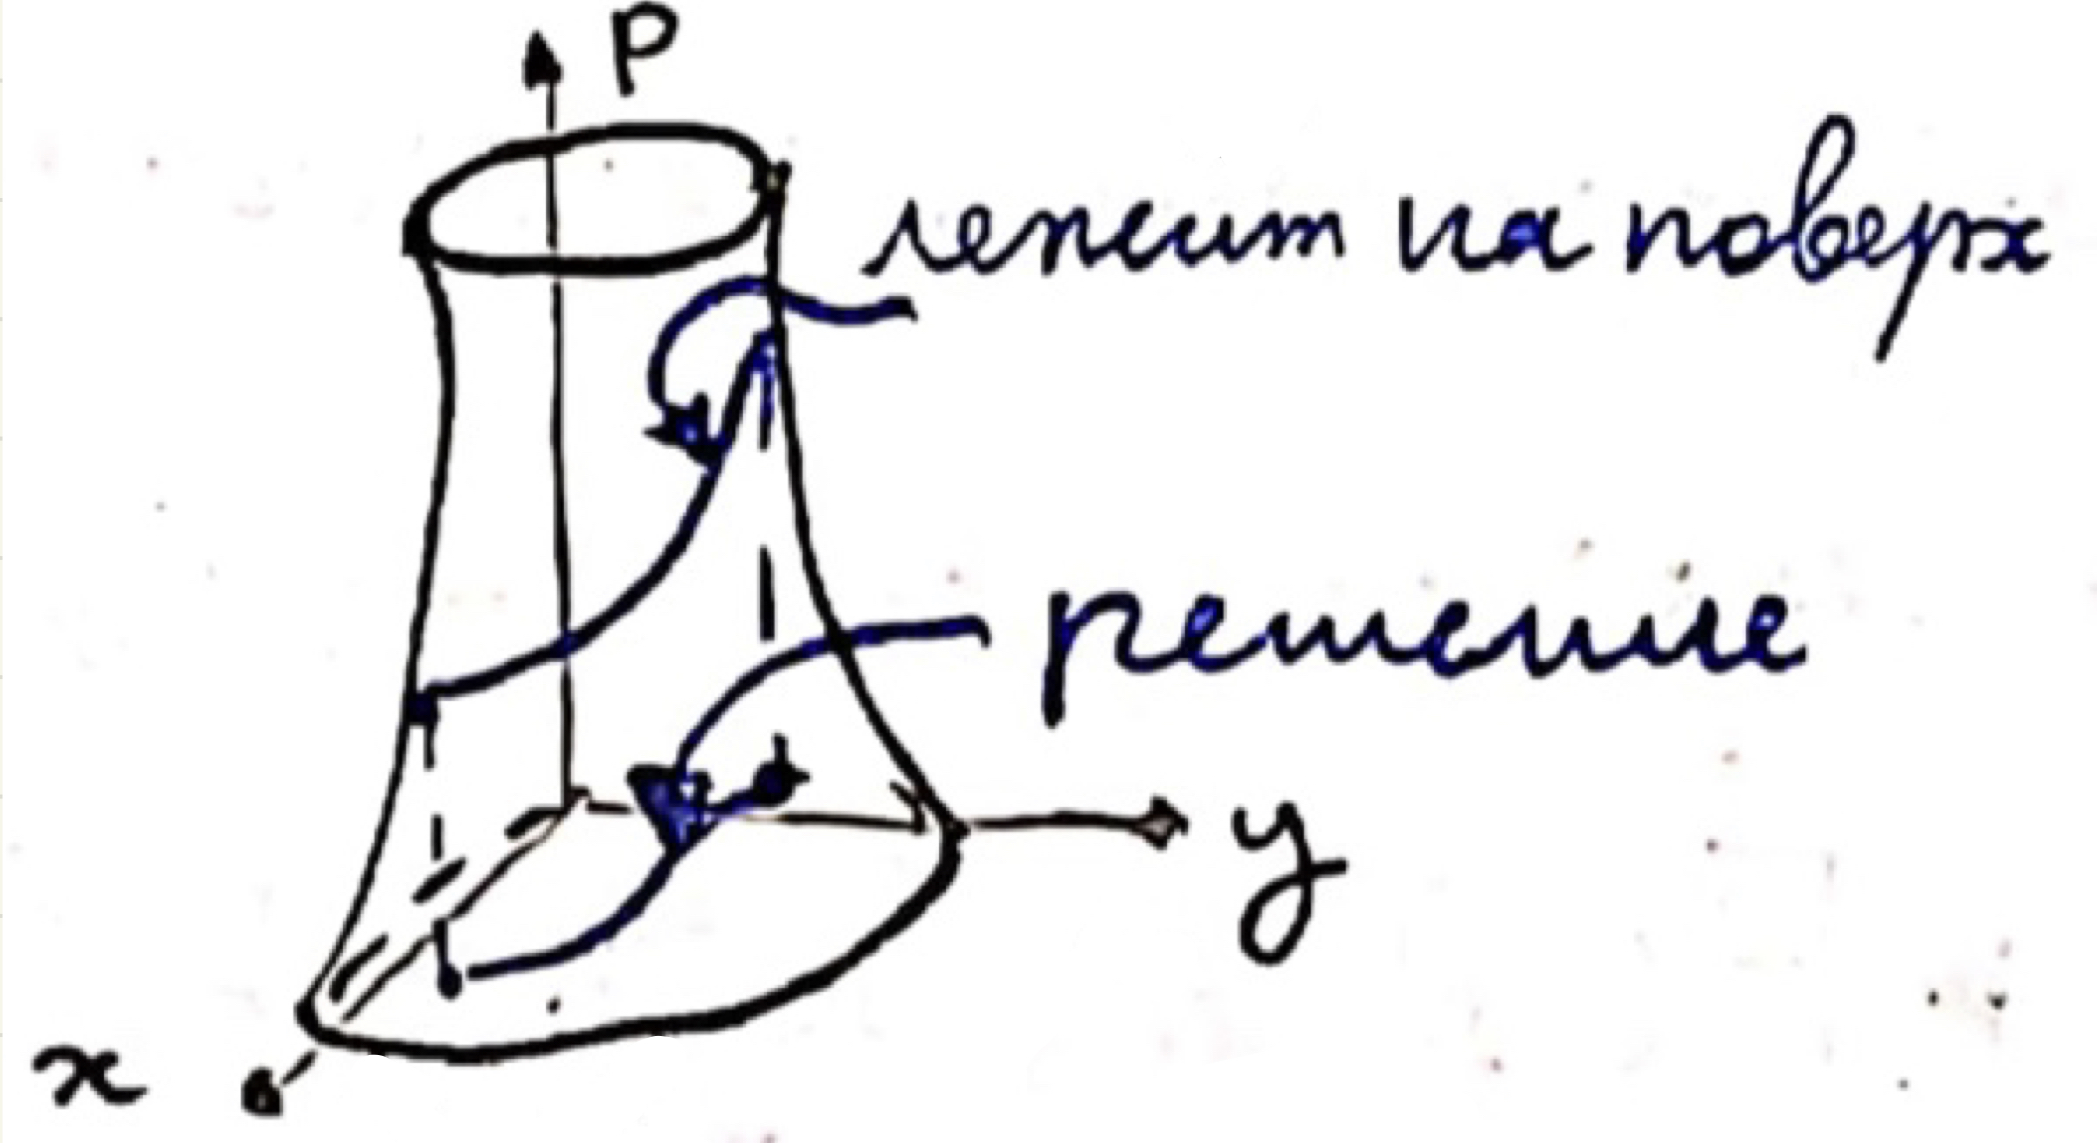
\includegraphics[width = 0.4\textwidth]{image_1.jpeg}
	\end{figure}	
	\[
	\left\{
	\begin{aligned}
		x &= \varphi(u, v)  \\
		y &= \psi(u, v) \\   
		p &= \chi(u, v) \\
	\end{aligned}
	\right. , (u, v) \in G
	\Rightarrow  F(\varphi(u, v), \psi(u, v), \chi(u, v)) \equiv 0                                               
	\]
	Потребуем, чтобы
	\[
		\text{rank}
		\begin{pmatrix}
			\dfrac{\partial\varphi}{\partial u} & \dfrac{\partial \psi}{\partial u} & \dfrac{\partial \chi}{\partial u} \\
			\\
			\dfrac{\partial\varphi}{\partial v} & \dfrac{\partial \psi}{\partial v} & \dfrac{\partial \chi}{\partial v}
		\end{pmatrix} = 2, \ \forall (u, v) \in G 
	\]
	т.е. чтобы $S$ была простой гладкой поверхностью.
	Тогда остаётся удовлетворить второму уравнению системы \eqref{eq:Fs}: \\
	\begin{equation} \label{eq:F6}
		\frac{\partial \psi}{\partial u} du + \frac{\partial \psi}{\partial v} dv = \chi \cdot \left(\frac{\partial \varphi}{\partial u}du + \frac{\partial \varphi}{\partial v}dv\right) \Rightarrow \left( \frac{\partial \psi}{\partial u} - \chi \frac{\partial \varphi}{\partial u} \right) du = \left(\chi \frac{\partial \varphi}{\partial v} - \frac{\partial \psi}{\partial v} \right) dv
	\end{equation}
	Если $ P(u, v) \neq 0 \ \forall (u, v) \in G$, то из \eqref{eq:F6} получаем ДУ: $ \dfrac{du}{dv} = \dfrac{Q(u, v)}{P(u, v)} $
	\[
		\text{Его решение} \  u = u(v, C),  \text{тогда } \left\{
		\begin{aligned}
			x &= \varphi(u(v, C), v) = x(v, C)  \ \text{ -- является параметрическим}\\
			y &= \psi(u(v, C), v) = y(v, C) \ \ \text{ представлением  решения \eqref{eq:F4}}\\   
		\end{aligned}
		\right.   
	\]
	\\ 
	Если же существует связь между $u$ и $v$: $ u = f(v), P(f(v), v) = Q(f(v), v) = 0 \ \forall v \in G$, то $ u = f(v) $ является решением $\left( \frac{\partial \psi}{\partial u} - \chi \frac{\partial \varphi}{\partial u} \right) du = \left(\chi \frac{\partial \varphi}{\partial v} - \frac{\partial \psi}{\partial v} \right) dv $, а 
	\[
	\left\{
	\begin{aligned}
		x &= x(v)\\
		y &= y(v)\\   
	\end{aligned}
	\right.   \
	\text{ -- является решением } \eqref{eq:F6}
	\]
\end{proposition}
    \newpage
    \section{Билет 2. Задача Коши}
\subsection{Принцип сжимающих отображений}

Работаем в $E =\mathbb{R}^n$ -- пространство точек с $n$ координатами. $E$ -- аффинное пространство, а $\vec{E}$ -- его присоединенное линейное пространство, состоящее из векторов, натянутых на точки $E$.

\begin{definition}
	Пусть $L$ -- это векторное пространство, и на нем задано отображение $\|\cdot\|:L\longrightarrow \mathbb{R}$ такое, что:
	\begin{enumerate}
		\item $\forall x \in L \longmapsto \|x\| \geqslant 0$. А также $\|x\| = 0 \Longleftrightarrow x = 0$;
		
		\item $\forall x \in L \; \& \; \forall \lambda \in \mathbb{R} \longmapsto \|\lambda x\| = |\lambda| \cdot \|x\|$;
		
		\item $\forall x, y \in L \longmapsto \|x+y\| \leqslant \|x\| + \|y\|$ -- неравенство треугольника.
	\end{enumerate}
	Тогда данное отображение называется нормой, а пространство $L$ нормированным.
\end{definition}

\begin{example}
	Приведем пример норм. Пусть $a(x_1, x_2, \dots, x_n) \in \mathbb{R}^n$. Тогда норму можно определить, допустим, так:
	\begin{equation}
		\|a\|_1 = \sqrt{\sum_{j = 1}^{n} x_j^2}.
	\end{equation}
Или так:
	\begin{equation}
		\|a\|_2 = \max_{j = 1, \dots, n}|x_j|.
	\end{equation}
\end{example}

И тогда можно ввести понятие эквивалентности норм.

\begin{definition}
	Пусть снова $L$ -- линейное пространство. Тогда нормы $\| \cdot \|_1$ и $\| \cdot \|_2$ на $L$ называются эквивалентными, если $\exists C_1, C_2 > 0: \; \forall x \in L \longmapsto C_1\|x\|_1 \leqslant \|x\|_2 \leqslant C_2\|x\|_1$.
\end{definition}

Как видно, для определенных выше двух норм это соотношение удовлетворяется.

\begin{proposition}
	В конечномерном линейном пространстве все нормы эквивалентны.
\end{proposition}

Рассмотрим множество функций, непрерывных на отрезке $[a; b]$ для некоторых неравных $a, b \in \mathbb{R}$ и обозначим данное множество $C[a; b]$. Понятно, что $C[a; b]$ является линейным пространством. Тогда введем на нем норму.

\begin{definition}
	Нормой функции $f(x) \in C[a; b]$ будем называть число $$\|f(x)\| = \max_{x \in [a; b]}|f(x)|.$$
\end{definition}

\begin{definition}
	Набор функций $f_1(x), f_2(x), \dots, f_n(x) \in C[a; b]$ будем называть вектор-функцией и обозначать $f(x) = \vec{f}(x) = \left(f_1(x), f_2(x), \dots, f_n(x)\right)^T$.
\end{definition}

\begin{definition}
	Вектор-функция $f(x)$ называется непрерывной (дифференцируемой, непрерывно дифференцируемой и т.п.), если все ее компоненты непрерывны (дифференцируемы, непрерывно дифференцируемы и т.п.).
\end{definition}

\begin{definition}
	Модулем вектор-функции $f(x)$ назовем число
	\begin{equation}
		|f(x)| = \sqrt{\sum_{j = 1}^{n} f_j^2(x) }.
	\end{equation}
\end{definition}

Норму вектор-функции можно определить как $$\|f(x)\|_1 = \max_{x \in [a; b]}|f(x)|.$$

Или же как $$\|f(x)\|_2 = \max_{j = 1, \dots, n} \max_{x \in [a; b]} f_j(x).$$

Понятно, что эти две нормы эквивалентны.

\begin{definition}
	Пусть имеется функциональная последовательность $\{f_n(x)\}_{n = 1}^{\infty}$, где $f_n(x) \in C[a; b]$ -- линейное пространство функций с нормой (1 или 2 -- неважно). Тогда говорят, что данная последовательность сходится к функции $f(x)$ по норме, если:
	\begin{equation}
		\lim\limits_{n\rightarrow \infty} \|f_n(x) - f(x)\| = 0.
	\end{equation}

Аналогично все то же самое и точно так же определяется и для вектор-функций $f(x) = \vec{f}(x) \in C^n[a; b]$.
\end{definition}

\begin{definition}
	Функциональная последовательность $\{f_n(x)\}_{n = 1}^{\infty}$ называется фундаментальной, если:
	\begin{equation}
		\forall \varepsilon > 0 \; \exists N \in \mathbb{N}: \; \forall n \geqslant N \; \& \; \forall m \geqslant N \longmapsto \|f_n(x) - f_m(x)\| < \varepsilon.
	\end{equation}
\end{definition}

\begin{definition}
	Функциональное пространство $L$ называется полным по [данной] норме, если любая фундаментальная функциональная последовательность данного пространства сходится по норме к функции из этого же пространства $L$.
\end{definition}

\begin{theorem}
	Функциональное пространство $C[a; b]$ с нормой $\| \cdot \|_1$ является полным.
\end{theorem}
\begin{proof}
	Возьмем произвольную функциональную последовательность $\{f_n(x)\}_{n = 1}^{\infty}$ из нашего пространства непрерывных функции. Тогда из определения фундаментальности следует, что $\|f_n(x) - f_m(x)\| < \varepsilon$.
	
	Однако $|f_n(x) - f_m(x)| \leqslant \|f_n(x) - f_m(x)\| < \varepsilon \; \forall x \in [a; b]$.
	
	А значит, последовательность $f_n(x)$ сходится к некоторой $f(x)$, причем равномерно на $[a; b]$ (числовая последовательность $\|f_n(x)\|$ мажорирует функциональную последовательность $f_n(x)$).
	
	Так как $f_n(x) \in C[a; b]$ -- непрерывны $\forall n \in \mathbb{N}$, и последовательность сходится равномерно на $[a; b]$, то предельная функция $f(x)$ также является непрерывной на $[a; b]$, а значит, $f(x) \in C[a; b]$. 
	
	Таким образом, последовательность $\{f_n(x)\}_{n = 1}^{\infty}$ сходится к $f(x) \in C[a; b]$. В силу произвольности $\{f_n(x)\}_{n = 1}^{\infty}$ заключаем, что функциональное пространство $C[a; b]$ с нормой $\| \cdot \|_1$ является полным.
\end{proof}

\begin{definition}
	Полное нормированное линейное пространство называется Банаховым. Обозначается $B$.
\end{definition}

\begin{definition}
	Функциональный ряд $\sum\limits_{k = 1}^{\infty} f_k(x)$ называется сходящемся по норме, если последовательность его частичных сумм $S_n(x) = \sum\limits_{k = 1}^{n} f_k(x)$ является сходящейся по норме.
\end{definition}

\begin{definition}
	Пусть $\forall x \in M \subseteq B$ определен элемент $Ax \in B$. Тогда говорят, что на множестве $B$ задан оператор $A$ с областью определения $M$.
\end{definition}

Будем рассматривать уравнение $x = Ax$.

\begin{definition}
	Множество $M \subseteq B$ называется ограниченным, если $\exists C > 0$ такое, что $\forall x \in M \longmapsto \|x\| \leqslant C$.
\end{definition}

\begin{definition}
	Оператор $A$ называется сжатием на $M$, если:
	\begin{enumerate}
		\item $\forall x \in M \longmapsto Ax \in M$;
		
		\item $\exists k \in (0; 1): \; \forall x, y \in M \longmapsto \|Ax - Ay\| \leqslant k\|x -y\|$.
	\end{enumerate}
\end{definition}

\begin{theorem}
	[Принцип сжимающих отображений]
	
	Пусть множество $M \subseteq B$, причём $M \neq \varnothing$, является ограниченным и замкнутым, а оператор $A$ является сжатием. Тогда решение уравнения $x = Ax$ существует и единственно.
\end{theorem}

\begin{proof}
	Будем использовать итерационный метод, согласно которому мы выбираем начальное $x_0$, а затем строим последовательность $x_n = Ax_{n-1}$. Тогда, если $\exists \lim\limits_{n \rightarrow \infty} x_n = x$ и $\exists \lim\limits_{n \rightarrow \infty} Ax_n = Ax$, то $x = Ax$.
	
		Пусть $x_n = S_n = x_0 + (x_1 - x_0) + \ldots + (x_n - x_{n-1})$.
		Докажем, что $\|x_{n+1} - x_n\| \leqslant 2Ck^n$ для некоторого $C > 0$, ограничивающего последовательность $x_n$. Сделаем это по индукции.
		
		База индукции: $\|x_1 - x_0\| \leqslant \|x_1\| + \|x_0\| \leqslant 2C$.
		
		Предположим, что $\|x_n - x_{n-1}\| \leqslant 2Ck^{n-1}$. Тогда получаем, что $\|x_{n+1} - x_n\| = \|Ax_n - Ax_{n-1}\| \leqslant k \|x_n - x_{n-1}\| \leqslant 2Ck^n$.
		
		Таким образом доказали, что $ \|x_{n+1} - x_n\| \leqslant 2Ck^n $.
		 $$\forall m,~ n: m > n \hookrightarrow \|x_m - x_n\| \leq \sum\limits_{j = n}^{m-1} {\|x_{j + 1} - x_j\|} = \sum\limits_{j = n}^{m-1} {2Ck^j} \leq 2Ck^n \frac{1}{1 - k} = a_n$$
		
	$\lim\limits_{n \to \infty}{a_n} = 0 \Rightarrow x_n - $ фундаментальная последовательность $\Rightarrow$ Поскольку $M$ -- полное $\exists \lim\limits_{n \rightarrow \infty} x_n = x$. Поскольку $M$ замкнуто, то $x \in M$. 
	
	(Пусть $\{z_m\} \subset M \Rightarrow \{z_m\} \subset M$. Пусть $\{z_m\} \to Z \subset B$. Поскольку $M - $ замкнутое, то содержит все свои предельные точки $\Rightarrow Z \subset M \Rightarrow M -$ полное)
		
		Рассмотрим $\|Ax_n - Ax\| \leqslant k\|x_n - x\| \underset{n \rightarrow \infty}{\longrightarrow} 0$. Это означает, что $\exists \lim\limits_{n \rightarrow \infty} Ax_n = Ax$. 
		
		Учитывая, что $x_{n+1} = Ax_n$, то, перейдя к пределу с обеих частей равенства, мы получаем, что итерационный метод сходится к решению уравнения $x = Ax$. И таким образом, доказано существование решения. Теперь докажем его единственность.
		
		Пойдем от противного: пусть $x$ и $y$ -- два разных решения. Тогда $\|x - y\| = \|Ax - Ay\| \leqslant k \|x - y\|$. Учитывая, что $k \in (0; 1)$, то данная ситуация возможна тогда и только тогда, когда $\|x - y\| = 0$. Следовательно, $x = y$, что противоречит тому, что это два разных решения. Итак, теорема доказана.
\end{proof}
    \subsection{Теорема существования и единственности решения задачи Коши для нормальной системы дифференциальных уравнений}

\begin{definition}
	Система вида
	\begin{equation}
		\label{equ:norm-sys}
		\begin{cases*}
			\dot{x}^1 = f^1(t, \bar{x}) \\
			\dot{x}^2 = f^2(t, \bar{x}) \\
			... \\
			\dot{x}^n = f^n(t, \bar{x})
		\end{cases*}
	\end{equation}
	называется нормальной системой дифференциальных уравнений n-ого порядка.
	
\end{definition}

\begin{definition}
	Система
	\begin{equation}
		\label{equ:init-cond}
		\begin{cases*}
			x^1(t_0) = x_0^1 \\
			x^2(t_0) = x_0^2 \\
			... \\
			x^n(t_0) = x_0^n
		\end{cases*}
	\end{equation}
	называется начальным условием
\end{definition}	

\begin{proposition}
	Решить задачу Коши означает решить нормальную систему дифференциальных уравнений при заданном начальном условии
\end{proposition}

\begin{theorem}[Теорема Коши о существовании и единственности решения]
	Пусть $\forall i, j \hm= \overline{1, n}$ функции $f^i, \dfrac{\partial{f^i}}{\partial{x^j}}$ непрерывны в области $\Omega \subset \mathbb{R}^{n+1}$, тогда, $\forall (t_0, \overline{x_0}) \in \Omega \text{ } \exists h>0 : \forall t \hm\in [t_0-h, t_0+h]$ решение задачи Коши существует и единственно.
\end{theorem}

\begin{lemma}
	Если $\bar{f}(t, \bar{x})$ - непрерывны на $\Omega$, то система уравнений
	\begin{equation}
		\label{equ:int-sys}
		\overline{x}(t) = \overline{x_0} + \int\limits_{t_0}^t\bar{f}(\tau, \overline{x}(\tau))d\tau
	\end{equation}
	эквивалентна задаче Коши.
\end{lemma}

\begin{proof}
	Пусть $\varphi(t)$ - решение (\ref{equ:norm-sys}) при условии (\ref{equ:init-cond}), тогда
	\[
		\dot{\varphi}^i = f^i(t, \varphi^1(t), \dots, \varphi^n(t))
	\]
	Проинтегрируем полученное равенство по отрезку $[t_0, t]$
	\begin{align*}
		&\int\limits_{t_0}^t \dot{\varphi}^i(\tau)d\tau = \int\limits_{t_0}^t f^i(\tau, \varphi^1(\tau), \dots, \varphi^n(\tau)) d\tau \\
		&\varphi^i(t) - \varphi^i(t_0) = \int\limits_{t_0}^t f^i(\tau, \bar\varphi(\tau))d\tau \\
		&\varphi^i(t) = x_0^i + \int\limits_{t_0}^t f^i(\tau, \bar\varphi(\tau))d\tau
	\end{align*}
	Теперь пусть $\bar{\varphi}(t)$ - решение (\ref{equ:int-sys}). Тогда
	\[
		\varphi^i(t) \equiv x_0^i + \int\limits_{t_0}^t f^i(\tau, \bar{\varphi}(\tau))d\tau
	\]
	Отсюда видно, что функция $\varphi^i(t)$ - дифференцируемы. Тогда
	\begin{equation}
	\begin{cases*}
		\dot{\varphi}^i(t) = f^i(t, \bar{\varphi}(t)) \\
		\varphi^i(t_0) = x_0^i
	\end{cases*}
	\end{equation}
\end{proof}

\begin{corollary}
	Из 2 части леммы следует, что решение задачи Коши непрерывно дифференцируемо.
\end{corollary}

Введем оператор $A(\bar{x}) = \bar{x}_0 + \int\limits_{t_0}^t \bar{f}(\tau, \bar{x}(\tau)) d\tau$. Тогда систему интегральных уравнений (\ref{equ:int-sys}) можно записать в виде 
\begin{equation}
	\label{equ:altern}
	\bar{x}(t) = A(\bar{x})
\end{equation}

\begin{lemma}
	\[
	\left\Arrowvert \int\limits_{t_0}^t\bar{x}(\tau)d\tau \right\Arrowvert \le \left\arrowvert \int\limits_{t_0}^t \Arrowvert \bar{x}(\tau)\Arrowvert d\tau \right\arrowvert
	\]
\end{lemma}

\begin{proof}
	\begin{equation}
		\left\arrowvert \int\limits_{t_0}^t x^i(\tau)d\tau \right\arrowvert \le\left\arrowvert \int\limits_{t_0}^t \left\arrowvert x^i(\tau) \right\arrowvert d\tau\right\arrowvert \le \left\arrowvert \int\limits_{t_0}^t \Arrowvert \bar{x}(\tau)\Arrowvert d\tau \right\arrowvert
	\end{equation}
	Таким образом $max\{|\int\limits_{t_0}^t x^i(\tau)d\tau|\} = || \int\limits_{t_0}^t \bar{x}(\tau)d\tau || \le \arrowvert \int\limits_{t_0}^t \Arrowvert \bar{x}(\tau)\Arrowvert d\tau \arrowvert$
\end{proof}

\begin{lemma} (Адамара)
	Пусть $\bar{f}(\bar{x}), \dfrac{\partial f^i}{\partial x_j}$ непрерывны в $\Omega \subset \mathbb{R} $ - замкнутой, ограниченной, выпуклой области. Тогда $\forall i = \overline{1,n}, \bar{y} \in \Omega \hookrightarrow \| \bar{f}(\bar{y}) - \bar{f}(\bar{x}) \| \le n^{3/2}K_1\|\overline{y-x}\|$, где $K_1 = max_{i,j=\overline{1,n}}\{max_{x\in\Omega}\left\{\left|\dfrac{\partial f^i}{\partial x_j}\right|\right\} \}$
\end{lemma}

\begin{proof}
	
	$|\bar{f}| = \sqrt{\sum\limits_{i=1}^n (f^i)^2}$, $\|\bar{f}\|_C = max_{x\in\Omega}\{|\bar{f}(\bar{x})|\}$
	
	$\Omega$ - компакт, поэтому непрерывность частных производных позволяет говорить о существовании $K_1$. Возьмем производные точки $\bar{x}$ и $\bar{y}$ и соединим их отрезком $\bar{x} + t(\bar{y} - \bar{x})$, где $t\in[0, 1]$. Рассмотрим значение компоненты $f^i$ на отрезке:
	\[
		f^i(\bar{x} + t(\bar{y} - \bar{x})) = f^i(t)
	\]
	$f^i(t)$ - дифференцируема, тогда
	\begin{align*}
		&|f^i(\bar{y}) - f^i(\bar{x})| = |f^i(1) - f^i(0)| = \left| \frac{df}{dt}(t^*)\cdot(1-0)\right| = \\
		&= \left|\sum\limits_{j=1}^n\frac{\partial f^i}{\partial x^j}(t^*)\cdot(y^j - x^j)\right| \le \sum\limits_{j=1}^n\left|\frac{\partial f^i}{\partial x^j}(t^*)\right|\cdot\left|(y^j - x^j)\right| \le K_1\|\bar{y}-\bar{x}\|\cdot n
	\end{align*}
	Теперь рассмотрим вектор-функцию
	\begin{align*}
		&|\bar{f}(\bar{y}) - \bar{f}(\bar{x})| = \sqrt{\sum\limits_{k=1}^n (f^k(\bar{y}) - f^k(\bar{x}))^2} \le K_1n^{3/2}\|\bar{y}-\bar{x}\| \\
		&\Rightarrow \|\bar{f}(\bar{y}) - \bar{f}(\bar{x})\| \le K_1n^{3/2}\|\bar{y}-\bar{x}\|
	\end{align*}
\end{proof}

\begin{proof}
	(Основная теорема)
	
	Докажем, что $A(\bar{x})$ из системы (\ref{equ:altern}) является сжатием.
	
	Рассмотрим $\Pi = \{\|\bar{x}(t) - \bar{x}_0(t)\| \le b, |t-t_0| \le a   \} \subset \Omega$. Определим $K = \|\bar{f}\|_C = max_{\Pi}|\bar{f}|$. $K_1$ тоже определено в силу условий.
	
	Рассмотрим $\Pi_h = \{\|\bar{x}(t) - \bar{x}_0(t)\| \le b, |t-t_0| \le h \le a   \}$
	
	Банахово пространство $B$ - множество функций $\bar{x}(t)$ непрерывных на отрезке $|t-t_0|\hm\le h$. $M \subset B$ - множество функций $\|\bar{x}(t) - \bar{x}_0\| \le b$. $M$ ограничено, так как $\forall \bar{x}(t) \in M \hookrightarrow \|\bar{x}(t)\| = \|\bar{x}(t) - \bar{x}_0 + \bar{x}_0\| \le b + \|\bar{x}_0\| = C$
	
	Докажем, что $M$ замкнуто. Пусть $\bar{x}_n(t), n = 1, 2, \dots$ - последовательность точек в $M$, такая что $\lim\limits_{n\to \infty} \bar{x}_n(t) = \bar{x}(t)$. $\|\bar{x}(t)\| = \|\bar{x}(t) - \bar{x}_n + \bar{x}_n\| \le \|\bar{x}(t) - \bar{x}_n\| + \|\bar{x}_n\| \le \varepsilon + b$ $\Rightarrow \bar{x}(t) \in M$
	
	Подберем $h$ так, чтобы $A:M\to M$. То есть $\|A(\bar{x}) - \bar{x}_0\| \le b$.
	\[
		\|A(\bar{x}) - \bar{x}_0\| = \|\int\limits_{t_0}^t \bar{f}(\tau, \bar{x}(\tau))d\tau\| \le |\int\limits_{t_0}^t \|\bar{f}\|d\tau| \le Kh
	\]
	Получаем условие $h\le b/K$
	
	Чтобы доказать, что $A$ - сжатие, рассмотрим норму
	\begin{align*}
		&\|A(\bar{y}) - A(\bar{x})\| = \|\int\limits_{t_0}^t(\bar{f}(\tau, \bar{y}(\tau)) - \bar{f}(\tau, \bar{x}(\tau)))d\tau\|\le \\ &\le |\int\limits_{t_0}^t \|\bar{f}(\tau, \bar{y}) - \bar{f}(\tau, \bar{x})\|d\tau| \le K_1n^{3/2}\|\overline{y-x}\|\cdot|\int\limits_{t_0}^td\tau| \le K_1hn^{3/2}\|\overline{y-x}\|
	\end{align*}
	Откуда второе условие: $h < \dfrac{1}{n^{3/2}K_1}$
	
	Тогда оператор $A$ будет сжатием. Соответственно решение задачи Коши существует и единственно.
	
\end{proof}

\subsection{Теорема существования и единственности решения задачи Коши для уравнения $n$-го порядка в нормальном виде}

\begin{definition}
	Уравнение вида
	\begin{equation}
		\label{equ:norm}
		y^{(n)} = f(x, y, \dots, y^{(n-1)})
	\end{equation}
	называется уравнением $n$-го порядка в нормальной форме.
\end{definition}

\begin{definition}
	Система
	\begin{equation}
		\label{equ:init-norm}
		\begin{cases*}
			y(x_0) = y_0\\
			y'(x_0) = y_0'\\
			\dots \\
			y^{(n-1)}(x_0) = y^{(n-1)}_0
		\end{cases*}
	\end{equation}
	называется начальным условием уравнения n-го порядка в нормальной форме.
\end{definition}

\begin{proposition}
	Решить задачу Коши означает найти такое решение (\ref{equ:norm}), которое удовлетворяет условию (\ref{equ:init-norm})
\end{proposition}

\begin{theorem}[Теорема Коши о существовании и единственности решения]
	Если $f, \dfrac{\partial f}{\partial y'}, \dots, \dfrac{\partial f}{\partial y^{(n-1)}}$ непрерывны в $\Omega \subset \mathbb{R}^{n+1}$, тогда $\forall (x_0, \bar{y}_0) \in \Omega \exists h > 0: \forall x\in [x_0 +h, x_0-h]$ решение задачи Коши существует и единственно.
\end{theorem}

\begin{proof}
	Введем следующие функции: $y(x) = v_1(x), y'(x) = v_2(x), \dots, y^{(n-1)}(x) \hm= v_n(x)$. Таким образом получаем систему уравнений в нормальной форме
	\begin{equation}
		\begin{cases*}
			\dfrac{dv_1}{dx} = v_2\\
			\dots\\
			\dfrac{dv_n}{dx} = f(x, \bar{v})
		\end{cases*}
	\end{equation}
	А для нее решение существует и единственно.
\end{proof}

    %% здесь должен быть Issue Ивана Старченко
    \newpage
    \section{Билет 3. Линейный дифференциальные уравнения и линейныесистемы диффуренциальных уравнений с постоянными коэффициентами}
    \section{Билет 3. Линейные дифференциальные уравнения и линейные системы дифференциальных уравнений с постоянными коэффициентами}

\subsection{Вводная часть}
\subsubsection{Понятие кольца. Рассмотрение понятия многочленов}

\begin{definition}
Кольцом $K$ называют множество, на котором определены две операции: сложение и умножение, сопоставляющее упорядоченным парам элементов их $"$сумму$"$, $"$произведение$"$, являющимся элементами этого же множества.
\end{definition}
Рассмотрим кольцо, в котором действия $+$ и $\cdot$ удовлетворяют следующим условиям (первые $6$ -- определение кольца):
\begin{enumerate}
    \item $(a+b)+c=a+(b+c)\;\;\;\forall a, b, c \in K$
    \item $a+b=b+a\;\;\;\forall a, b\in K$
    \item $\exists 0\in K:\;\;\; a+0=a \;\;\;\forall a\in K$
    \item $\forall ~ a ~ \in ~ K ~ \exists -a ~ \in ~ K: a+(-a)=0 ~ \forall a ~\in ~ K$
    \item $(a+b) \cdot c = ac + bc \;\;\; \forall a, b, c \in K$
    \item $c\cdot(a+b)=ca+cb\;\;\; \forall a, b, c\in K$
    \item $(ab)c=a(bc)\;\;\; \forall a, b, c\in K$
    \item $ab=ba \;\;\;\forall a, b\in K$
    \item $\exists 1\in K: a\cdot 1 =1\cdot a = a\;\;\;\forall a\in K$
    \item $\exists a^{-1} \in K: a^{-1}a=aa^{-1}=1\;\;\;\forall a\in K$
\end{enumerate}
\begin{proposition}
Если $a+x=a+y$, то $x=y$
\end{proposition}
\begin{proof}
$$(-a)+(a+x)=(-a)+(a+y)\Rightarrow \big((-a)+a\big) +x= \big((-a)+a\big) +y=0+x=x=0+y=y$$
Отсюда следует единственность нуля и противоположного элемента:
$$(-a)\neq (-a)'$$$$0=a+(-a)=a+(-a)'\Rightarrow(-a)=(-a)'$$
\end{proof}
\begin{proposition}
$a\cdot 0=0\cdot a=0 \;\;\;\forall a$
\end{proposition}
\begin{proof}
$a \cdot 0+0=a \cdot 0 = a(0+0) \Rightarrow a \cdot 0 =0$; аналогично $0+0 \cdot a=0 \cdot a=(0 + 0) \cdot a =0 \cdot a + 0 \cdot a \Rightarrow 0 \cdot a =0$
\end{proof}
\begin{proposition}
Единица единственна
\end{proposition}
\begin{proof}
Пусть $1\neq1': 1=1\cdot 1'=1'\cdot 1=1'$
\end{proof}
\begin{itemize}
    \item Кольцо называется ассоциативным, если выполнено условие 7; коммутативным, если выполненно 8. Если выполнено условие 9, то говорят о кольце с единицей.
    \item Ассоциативное кольцо называется областно целостным, если из $ab=0\Rightarrow a=0\bigvee b=0$
    \item Полем называется коммутативное ассоциативное кольцо с единицей, в котором каждый отличный от нуля элемент имеет обратный. 
    
\end{itemize}
\begin{proposition}
Любое поле является областно целостным
\end{proposition}
\begin{proof}
$ab=0, \;\;a \neq 0 \Rightarrow a^{-1} \cdot (ab)=a^{-1} \cdot 0=0=(a^{-1}a) \cdot b=1 \cdot b =b \Rightarrow b=0$
\end{proof}
\subsubsection{Многочлен}
Пусть $A~-~$коммутативное ассоциативное кольцо с единицей. Одночленом от $x$ с коэффициентом из $A$ называется выражение $ax^m, \;\;a\in A, \;\;m\in \mathbb{N}$. По определению положим, что $ax^0=a$. Выражение $ax^m$ будем рассматривать как символ, для которого выпоняется по определению: $$ax^m+bx^m=(a+b)x^m$$
$$ax^m\cdot bx^n= a \cdot b x^{m+n}$$
Выражение, состоящее из нескольких одночленов, соединенных знаком $+$ назовем многочленом от $x$ с коэффициентами из $A$. Без нарушения общности, в силу коммутативности сложения запишем в каноническом виде: $P_n(x)=a_0+a_1x+\dots+a_nx^n$
\begin{enumerate}
    \item\label{1} Многочлены $P_n(x)=a_0+a_1x+\dots+a_nx^n$ и $Q_m(x)=b_0+b_1x\dots+b_mx^m $ считаем равными в том и только в том случае,  если $n=m$ и $a_k=b_k, \;\;\;k=\overline{1, n}$
    \item Суммой двух многочленов $P_n(x)$ и $Q_n(x)$ называется многочлен, получившейся посредством объединения одночленов соответствующих слагаемых:$$P(x)+Q_m(x)=(a_0+a_1x+\dots+a_nx^n)+(b_0+b_1x^1+\dots+b_mx^m)=a_0+b_0+ (a_1+b_1)x+\dots+c_sx^s$$ 
    $$x=max\{n, m\} $$
    $c_s=a_s+b_s, a_s=0, $ если $s>n$ и $b_s=0, $ если $s>m$\par Так определенное сложение многочленов коммутативно и ассоциативно.\par Имеется нулевой элемент $0=0 \cdot x + \dots + 0 \cdot x^n, $ а также противоположный $\big(-P_n(x)\big)=(-a_0)+(-a_1)x++\dots+(-a^n)x^n$
    \item Произведением двух многочленов называют многочлен, составленный их произведения всех членов первого сомножителя на все члены второго.
    $$P_n(x)\cdot Q_m(x)=a_0b_0+(a_0b_1+a_1b_0)x+\dots+\Big(\displaystyle\sum_{j=k+l}a_kb_l \Big)x^j+\dots+a_nb_mx^{n+m}$$
    
\end{enumerate}
\begin{itemize}
    \item Покажем, что так определенное умножение будет коммутативно и ассоциативно:
    $$P_n(x)\cdot Q_m(x)=a_0b_0+(a_0b_1+a_1b_0)x+\dots+\Big(\displaystyle\sum_{j=k+l}a_kb_l \Big)x^j+\dots+a_nb_mx^{n+m}$$
    В сумме $\displaystyle\sum_{j=k+l}a_kb_l $ заменим $k\leftrightarrow l\Rightarrow \displaystyle\sum_{j=k+l}b_ka_l=\displaystyle\sum_{j=k+l}b_la_k=\displaystyle\sum_{j=k+l}a_lb_k\underset{(\ref{1})}{\Rightarrow}P_n(x)\cdot Q_m(x)=Q_m(x)\cdot P_n(x)\Rightarrow$ коммутативно.\par
    Пусть $R_s(x)=c_0+c_1x+\dots+c_sx^s\Rightarrow(P_n(x)\cdot Q_m(x))\cdot R_s(x)= \big((a-0)b_0)c_0\big)+\Big(\displaystyle\sum_{\gamma=j+\sigma}\Big(\displaystyle\sum_{j=k+l}a_kb_l\Big)c_\sigma\Big)x^\gamma + (a_nb_m)c_Sx^{n+m+s}), \;\;\;j=1, \dots, n+m+s-1$. Так как $\displaystyle\sum_{\gamma=j+\sigma}\Big(\displaystyle\sum_{j=k+l}a_kb_l\Big)c_\sigma = \displaystyle\sum_{\gamma=k+l+\sigma}a_k(b_lc_\sigma)$.
    
    Пусть $l'=l+\sigma\Rightarrow\displaystyle\sum_{\gamma=k+l+\sigma}a_k(b_lc_\sigma) =\displaystyle\sum_{\gamma=k+l'}a_k\Big(\displaystyle\sum_{l'=l+\sigma}b_lc_\sigma\Big)$ 
    $\underset{(\ref{1})}{\Rightarrow} (P_n(x)\cdot Q_m(x) )R_s(x)=P_n(x)\cdot(Q_m(x)\cdot R_s(x)))~-~$ ассоциативно.
    \item Дистрибутивность аналогично (везде используются свойства одночленов)\par Таким образом так построенное множество многочленов от $x$ над $A$ будет ассоциативным и коммутативным кольцом $A(x)$. Роль единицы в $A(x)$ играет единица их $A$.\par
    При построении кольца многочленов вместо $x$ положим $p=\frac{d}{dx}~-~$ оператор дифференцирования, который действует на множестве бесконечно дифференцируемых комплекснозначных функций. $p\cdot f(x)=p(f(x))=\frac{df}{dx}=f', \;\;p^2(f)=f'', \dots, p^nn(x)=f^{(n)};$ Справедлива формула $p^s\cdot p^m(f)=p^s\cdot (p^m(f))=p^s\cdot (f^{(m)})=f^{(m+s)}=p^{m+s}(f)$.\par
    По определению, множество бесконечно дифференцируемых комплекснозначных функций $\varPhi$ является кольцом, содержащим поле $\mathds{C}$. В качестве элементов кольца $A$ будем брать  числа из $\mathds{C}$.
    Роль операторного одночлена в таком случае будет играть $ap^m, \;\;a\in\mathds{C};\;\;ap^m=p^ma, $ так как $ap^m(f)=af^{(m)}=f^{(m)}\cdot a = p^m(f)\cdot a;$ По определению положим $ap^0=a, $ что корректно, так как $ap^0f=ap^0(f)=af=a\cdot f=a(f).$ Приведение подобных слагаемых для одночленов определим как $ap^m+bp^m=(a+b)p^m$, поскольку $(ap^{(m)})(f)+bp^{(m)})(f)=af^{(m)}+b^{(m)}=(a+b)f^{(m)}=((a+b)p^m)(f)$.\par
    Аналогично вводим выражение, состоящее из нескольких операторных одночленов, соединенных знаком $+$, называемое операторным многочленом от $p$ с коэффициентом из $\mathds{C}$. Из свойств дифференцирования следует, что в общем виде можно записать $L_n(p)=a_0+a_1p+\dots+a_np^n$\par
    Абсолютно аналогично доказываем, что замена $x$ на $p$ дает множество операторных многочленов от $p$, которое будет кольцом из $\mathds{C}$
    \item Пусть $x \in \mathds{C}$. Значение многочлена $P_n(x)$ на $\mathds{C}$ определим как число $P_n(x) = a_0 + a_1 z + \dots + a_n z^{n} \in \mathds{C}$. \par
    Понятие значения многочлена можно обобщить на случай, когда $B$ является ассоциативным кольцом, содержащим кольцо $A$, в случае, когда элементы $A$ коммутируют с элементами из $B$.\par
    В таком случае можно определить степень элемента кольца $B$. Пусть $a\in B, \;\;a^1=a, \;\;a^2=a\cdot a, \dots, a^n=a^{n-1}\cdot a$
    \begin{theorem}
    $\forall k\in \mathbb{N}, \forall m \in \mathbb{N} \rightarrow a^k\cdot a^m= a^{k+m}$
    \end{theorem}
    \item Значение операторного многочлена $L_n(p) $ определим на коммутативном и ассоциативном кольце $\varPhi~-~$ бесконечно дифференцируемой комплекснозначной функцией от $x \in \mathbb{R}: \;\;f(x)$$$L_n(F)=L_n(p)(f)=a_0f+a_1f'+\dots+a_nf^{(n)}\in \varPhi$$
    \item Если $F(p)=L_n(p)+M_m(p)$ определим сумму на множеcтве дифф. операторов:$$F(p)=(a_0+b_0)f+(a_1+b_1)f'+\dots+c_sf=L_n(p)(f)+M_m(p)(f)\Rightarrow (L_n(p)+M_m(p))(f) =$$ 
    $$=(M_m(p)+N_m(p))(f)$$ коммутативно, ассоциативность аналогично.
    \item $(L_n(p) M_m(p))(f)=(a_0 b_0 p^0 + (a_0 b_1 + a_1 b_0)p+ \dots + \left(\displaystyle \sum_{j=k+l}a_kb_l \right)p^j+ \dots +a_n b_m p^{m+n})(f)=a_0 b_0 f +(a_0 b_1 + a_1 b_0)f'+ \dots +(\displaystyle \sum_{j=k+l} a_k b_l)f^{(j)}+ \dots +a_n b_m f^{(n+m)} = (a_0 p^0 + a_1 p+ \dots + a_n p^n) \cdot (b_0 f + b_1 f'+ \dots + b_m f^{(m)})=\;L_n(p) \cdot (M_m(f))~-~$ определение действия произведения операторов на множестве $\varPhi$. Так как $a_0b_0 f+(a_0b_1+a_1b_0)f'+\dots+ \left(\displaystyle \sum_{j=k+l}a_kb_l \right)f^{(j)}+ \dots + a_n b_m f^{(m+n)} = M_m(p) \cdot (a_0 f+a_1 f' + \dots a_n f^{(n)})\Rightarrow (L_n(p)\cdot M_m(p))=\;\;=(M_m(p)\cdot L_n(p)) ~-~$ коммутативность.
    \item Покажем ассоциативность и дистрибутивность
    $$ L_n(p)\cdot M_m(p)K_s(p)(f) = (L_n(p)\cdot M_m(p))(K_s(p)(f)) = $$ $$ = L_n(p)(M_m(p)(K_s(p)(f)))= L_n(p)(Q_m(p)R_s(p))(f) $$
    
    ассоциативность. $$(L_n(p)+M_m(p)K_s(p))(f)=L_n(p)(K_s(p)(f))+M_m(p)(K_s(p)(f))= $$ 
    $$ = (L_n(p)K_s(p))(f)+(M_m(p)K_s(p))(f)$$дистрибутивность $\cdot $ и $+$.\par
    Таким образом, множество значений операторных многочленов является кольцом, которое содержится в $\varPhi$.
    \item Если для $P_n(x)$ и $Q_m(x)$ из $A(x)\;\;\;\exists R_s(x)\in A(x): \;\;P_n(x)=Q_m(x)\cdot R_s(x), $ то говорят, что $P_n(x)$ делится на $Q_m(x)$.
    \begin{theorem}
    $$P_n(x) = a_n x^n + a_{n-1} x^{n-1} + \dots + a_0 \in A(x), \;c \in A \Rightarrow \exists ! Q_m(x),  r\in \mathds{C}:P_n(x)=(x-c)Q_m(x)+r$$.
    \end{theorem}
    \begin{theorem}
    (Безу) $P_n(x)$ делится на $x-c\Leftrightarrow P_n(c)=0$.
    \end{theorem}
    \begin{theorem}
    Если кольцо $A$ является областью целостности, то число корней $P_n(x)$ не превосходит $n$.
    \end{theorem}
    \begin{theorem}
    Основная теорема алгебры \par
    Любой многочлен $P_n(x)$ над $\mathds{C}$ имеет хотя бы один корень.
    \end{theorem}
    \begin{proposition}
    Из $3$ и $5$ теоремы \begin{equation}
        \forall P_n(x)\rightarrow P_n(x)=a_n(x-c_1)^{l_1}\cdot \dots
    \cdot (x-c_k)^{l_k} 
    \end{equation}
    \end{proposition}
    \item Взаимнооднозначное соответствие $\varphi$ кольца $K$ на кольцо $K'$ называется изоморфизмом, если $\forall a\in K $ и $\forall b\in K'\rightarrow$
    \begin{equation}
        \label{3}
        \varphi(a+b)=\varphi(a)+\varphi(b)\;\;\;\;\;\;\;\varphi(a\cdot b)=\varphi(a)\cdot\varphi(b)
    \end{equation}
    Из $\eqref{3}$ следует, что образом нуля кольца $K$ будет нуль $K$: $\varphi(a)=a'\in K'$ и $\varphi(0)=c',\;\;\varphi(a)=a'=\varphi(a+o) = \varphi(a)+\varphi(0)=a'+c'\Rightarrow c'=0$\par
    Если кольцо $K$ имеет единицу, то $\varphi(1)$ будет единицей кольца $K'$: $\varphi(a)=a'=\varphi(1\cdot a )= \varphi(1)\cdot \varphi(a) = \varphi(1) a'\Rightarrow\varphi(1)~-~$ единица $K'$.
    \item Обратное отображение $\varphi^{-1}$ кольца $K'$ на $K$ существует и будет изоморфно.\par
    Рассмотрим отображение $\varphi,$ которое множеству значений $P_n(x)$ над $\mathds{C}$ ставит в соответствие множество значений $L_n(p)$ на множестве бесконечно дифференцируемых комплекснозначных функций $\varPhi$ по принципу:
    $$\varphi(P_m(z))=\varphi(a_nz^n+a_{n-1}z^{n-1}+\dots+a_0z^0)=L_n(p)(f)=a_nf^{(n)}+a_{n-1}f^{(n-1)}+\dots+a_0f;$$
    Покажем, что отображение является изоморфизмом.\par Отображение взаимнооднозначно по построению.
    $$\varphi(P_n(z)+Q_m(z))=\varphi(a_0+a_1z+\dots+a_nz^n+b_0+b_1z+\dots+b_mz^m)=$$
    $$=\varphi(a_0+b_0+(a_1+b_1)z+\dots+(a_s+b_s)z^s)=$$
    $$=(a_0+b_0+(a_1+b_1)p+\dots+(a_s+b_s)p^s)(f)=L_n(p)+L_m(p)(f)$$
    $$\varphi(P_n(z)\cdot Q_m(z))=\varphi(a_0b_0+\displaystyle\sum_{j=k+l}a_kb_lz^j+a_nb_mz^{m+n})=$$
    $$=(a_0b_0+\displaystyle\sum_{j=k+l}a_kb_lp^j+a_nb_mp^{m+n})=L_n(p)\cdot Q_m(p)(f)$$
    Таким образом, $\varphi~-~$изоморфизм. Тогда из $(\ref{3})$: $$\varphi(P_n(x))=\varphi(a_n(z-c_1)^{l_1}\cdot ...\cdot (z-c_k)^{l_k})= L_n(p)(f)=a_n\cdot (p-c_1)^{l_1}\cdot ... \cdot я(p-c_k)^{l_k}(f)$$
    В итоге  $L_n(p)=a_n\cdot (p-c_1)^{l_1}\cdot ... \cdot (p-c_k)^{l_k},$ где $c_1, \dots, c_k ~-~$ корни $P_n(z)$.
    
\end{itemize}
\subsection{Линейные уравнения с поcтоянными коэффициентами}
Рассмотрим ДУ вида: $a_n y^{(n)}+a_{n-1}y^{(n-1)} + \cdots +a_0y=0, \;\;\;a_n \neq 0, $ где $a_i=const\;\;\forall i=\overline{1, n}.$ Через введенный ранее дифференциальный оператор $L_n(p)=a_np^n+ \dots + a_0 p^0$ уравнение записывается в виде \begin{equation}\tag{2.1}
\label{2.1}
    L_n(p)(y(x))=0
\end{equation}
Было доказано, что $L_n(p)$ является изоморфизмом характеристического многочлена $(\ref{2.1})$: $P_n(\lambda)=a_n\lambda^n+\dots+a_0=a_n(\lambda-\lambda_1)^{l1}\cdot ... \cdot (\lambda-\lambda_{k})^{l_k}$ и поэтому для $L_n(p)$ справедливо разложение \begin{equation}
    \tag{2.2}
    \label{2.2}
    L_n(p)=a_n(p-\lambda_1)^{l1}\cdot ... \cdot (p-\lambda_{k})^{l_k}, \;\;\;p=\frac{d}{dx}
\end{equation}
Задача: найти ФСР $(\ref{2.1})$. Из записи $L_n(p)$ ясно, что решением$ (\ref{2.1})$ будут функции из $\varPhi$, котрые являются корнями $L_n(p)$.
\begin{lemma}
Для любой $n$ раз дифференцируемой на промежутке функции $f(x)$, $\lambda\in\mathds{C}$ выполняется "формула сдвига" \begin{equation}
    \tag{2.3}
    \label{2.3}
    L_n(p)(e^{\lambda x}f)=e^{\lambda x}\cdot L_n(p+\lambda)(f)
\end{equation}  
\end{lemma}
\begin{proof}
Докажем по индукции. База $n=1$: $$L_1(p)(e^{\lambda x}f)=(a_1p^1+a_0)(e^{\lambda x}f)=e^{\lambda x}(a_0f+a_1(\lambda f+ f'))=e^{\lambda x}(a_1(p+\lambda)+a_0)(f)=e^{\lambda x}L_1(p+\lambda)(f)$$
Пусть $(\ref{2.3})$ справедлива для $k=n-1$, то есть $L_{n-1}(p)(e^{\lambda x} f)=e^{\lambda x} L_{n-1}(p+\lambda)(f)$\par
Обозначим $L_n(p)=p-\lambda_1,$ тогда по формуле $(\ref{2.2}):$
$$L_n(p)=a_n(p-\lambda_1)\cdot (p-\lambda_1)^{l_1-1}\cdot ...\cdot (p-\lambda_m)^{l_m} \cdot ... \cdot (p-\lambda_k)^{l_k}=L_1(p)\cdot L_{n-1}(p)=L_{n-1}(p)\cdot L_1(p)$$
Тогда $L_n(p)(e^{\lambda x }f) = L_{n-1}(p) \cdot L_1(p)(e^{\lambda x}f(x))=L_{n-1}(p)(L_1(p)(e^{\lambda x}f))\underset{\text{база}}{=} L_{n-1}(p)(e^{\lambda x}\cdot (p+\lambda) (f))$\par
Обозначим через $g(x)=L_1(p+\lambda)(f(x)),$ имеем:

$$L_n(p)(e^{\lambda x}f) = L_{n-1}(p)(e^{\lambda x}g(x))\underset{\text{индукция}}{=}e^{\lambda x}L-{n-1}(p+\lambda)(g) = $$ $$ = e^{\lambda x}L_{n-1}(p+\lambda)(L_1(p+\lambda)(f))=e^{\lambda x}(L_{n-1}(p+\lambda)\cdot L_{1}(p+\lambda))(f)=e^{\lambda x}\cdot L_n(p+\lambda)(f(x))$$

\end{proof}
\begin{theorem}
Если $\lambda_m$ является корнем $L_n(\lambda)$ кратности $l_m,$ то функции $e^{\lambda_m x}, xe^{\lambda_m x}, \dots$, $x^{l_m-1}e^{\lambda_m x}$ являются решениями $(\ref{2.2})$
\end{theorem}
\begin{proof}
Из коммутативности и ассоциативности кольца операторных многочленов и формулы $(\ref{2.3})$: $L_n(p)=a_n(p-\lambda_1)^{l_1}\cdot ... \cdot (p-\lambda_m)^{l_m}\cdot ... \cdot (p-\lambda_k)^{l_k}=L_{n-l_m}(p)(p-\lambda_m)^{l_m}$\par
Воспользуемся формулой сдвига для $x^se^{\lambda_m x}:$
$$L_n(p)(x^se^{\lambda_m x})=e^{\lambda x}\cdot L_{n-l_m}(p+\lambda_m) \cdot p^{l_m}(x^s)=$$
$$=e^{\lambda_m x}\cdot L_{n-l_m}(p+\lambda_m)(x^s)^{(l_m)}=\left\{\begin{gathered}
    0, \;\;\forall s\leqslant l_{m-1}\hfill
    \\
    e^{\lambda_m x}\cdot P_{n-l_m}(x), s\geqslant l_m \hfill
    \\
\end{gathered}
\right.,$$
где $P_{n-l_m}$ многочлен степени не ниже $n-l_m$.\par
Таким образом $x^se^\lambda_m x, \;\;\;s=\overline{q, l_{m-1}}$ являются корнями $L-n(p),$ а значит и решениями$(\ref{2.1})$
\end{proof}
Из доказанной теоремы следует:
\begin{equation}
\tag{2.4}
\label{2.4}
    \Bigg\{\{e^{\lambda_1 x}, \dots, x^{l_1-1}e^{\lambda_1 x}\}, \dots, \{e^{\lambda_mx}, \dots, x^{l_m-1 }e^{\lambda_mx}\}, \dots, \{e^{\lambda_k x}, \dots, x^{l_k-q}e^{\lambda_k x}\}\Bigg\}
\end{equation}
будут решениями $(\ref{2.2})$. Всего таких функций $n$ штук. Докажем линейную независимость систем функций $(\ref{2.4})$.
\begin{lemma}\label{lem1}
Система $1, x, \dots, x^m$ линейно независима. 
\end{lemma}

\begin{proof}
Рассмотрим линейную комбинацию функций $C_0+C_1x+\dots+C_nx^n=0$\par От противного: пусть $\exists C_0, \dots, C_n:\;\;\;\displaystyle\sum_{i=0}^n C_i^2\neq0: C_0+C_1x+\dots+C_nx^n=0\;\;\;\forall x $\par Так как у многочлена степени $n$ не более чем $n$ нулей, то получаем противоречие.
\end{proof}
\begin{theorem}
Система функций $P_{n1}(x)e^{\lambda_1 x},\dots, P_{ns}(x)e^{\lambda_s x}, $ где $P_{ni}(x)$ является многочленом степени $n_i$,  а все $\lambda_i \in \mathds{C}$ разные,  является ЛНЗ.
\end{theorem}
\begin{proof}
Выражение $P_n(x)e^{\lambda x}~-~$квазимногочлен степени $n$, $\lambda\in\mathds{C}$, коэффициенты $P_n(
x)\in\varPhi$
Рассмотрим $(P_n(x)e^{\lambda x})'=\lambda\cdot P_n(x)e^{\lambda x}+e^{\lambda x}\overline{P}_{n-1}(x)=e^{\lambda x }(\lambda P_n(x)+\overline{P}_{n-1}(x))= \widetilde{P}_n(e^{\lambda x})$.\par То есть, если будем дифференцировать степень $n$, то останемся в множестве квазимногочленов степени $n$.\par
Докажем по индукции. База $n=1~-~$ выполнена по Лемме ($\ref{lem1}$). Пусть выполнено для $n=s-1:$ система из $s-1$ квазимногочленов является ЛНЗ системой: $P_{n_1}(x)e^{\lambda_1x}, \dots, P_{n_{s-1}}~-~$ ЛНЗ.\par
Для $n$. От противного: пусть система $P_{n_1}(x)e^{\lambda_1x}, \dots, P_{n_{s-1}}, P_{n_s}(x)e^{\lambda_s x}$ является линейно зависимой, тогда $\exists C_1, \dots, C_l, \dots, C_s:$
\begin{equation}
    \tag{2.5}
    \label{2.5}
    C_1P_{n_1}(x)e^{\lambda_1x}+C_2P_{n_2}(x)e^{\lambda_2x}+\dots+C_lP_{n_l}(x)e^{\lambda_lx}+\dots+C_sP_{n_s}(x)e^{\lambda_s}x=0
\end{equation}
и хотя бы одна константа, например $C_l\neq0$ Из $(\ref{2.5})$, перенося $C_l$ вправо и деля на $C_le^{\lambda_lx}$ получаем:
$$\overline{C_1}P_{n_1}(x)e^{\omega_1x}+\dots+\overline{C_s}P_{n_s}(x)e^{\omega_sx}=-P_{n_l}(x)$$ где $\overline{C_i}=\frac{C_i}{C_l\neq0}, \omega_i=\lambda_i-\lambda_l$.\par Продифференцируем $n_{l+1}$ раз последнее тождество. Перенумеровав $s-1$ слагаемое в левой части получим $\overline{C}_1\cdot \widetilde{P}_n(x)e^{\omega_1x}+\dots+\overline{C}_{s-1} \cdot \widetilde{P}_{n_{s-1}}(x)e^{\omega_{s-1}x}=0$.\par По определению индукции последнее равенство возможно, только если  все $\overline{C}_i=0, \;\;\overline{C}_i=\frac{C_i}{C_l};C_l\neq 0 \Rightarrow C_i =0, i=1, \dots, l-1, l+1, \dots, s\underset{(\ref{2.5})}{\Rightarrow} C_l=0~-~$ противоречие рпедположению индукции о линейносй независимости системы $P_{n_1}(x)e^{\lambda_1x}, \dots, P_{n_{s-1}}(x)e^{\lambda_{s-1}x}$.
\end{proof}
Таким образом ФСР дифференциального уравнения $(\ref{2.1})$ будет состоять из функций набора
$$ \Bigg\{\{e^{\lambda_1 x}, \dots , x^{l_1-1}e^{\lambda_1 x}\}, \dots, \{e^{\lambda_mx}, \dots, x^{l_m-1 }e^{\lambda_mx}\}, \dots, \{e^{\lambda_k x}, \dots, x^{l_k-q}e^{\lambda_k x}\}\Bigg\},$$
где $\lambda_1, \dots, \lambda_m, \dots, \lambda_k~-~$ корни характеристического многочлена $P_n(\lambda)$ кратности $l_1, \dots$, $l_m, \dots, l_k$.\par
Общее решение $(\ref{2.1})$ будет иметь вид
\begin{equation}
    \tag{2.6}
    \label{2.6}
    y_0=e^{\lambda_1x}\Big(\displaystyle\sum_{m=1}^{l_1-1}C_m^1x^m\Big)+\dots+e^{\lambda_kx}\Big(\displaystyle\sum_{m=1}^{l_k-1}C_m^kx^m\Big)
\end{equation}
Фигурирующие в $(\ref{2.6})$ константы $C_i^j$, вообще говоря, могут быть комплексными, если корни $P_n(\lambda)$ являются комплекснозначными. Если изначально ставится задача $~-~$ найти решение ДУ во множестве действительных функций действительного переменного, то в случае комплексных корней возникает задача выделить из множества комплексных решений действительное. Это осуществимо, так как коэффициенты $P_n(\lambda)$ являются действительными числами.\par
Пусть $\lambda_m=\alpha+\beta i ~-~$ корень характеристического многочлена кратности $i$. Ему соответствуют $\varphi_m^i=x^ie^{\alpha x}(\cos{\beta x}-i\sin{\beta x});\;\;\;\varphi^i_m, \overline{\varphi}_m^i~-~$ ЛНЗ, $i=\overline{0, l-1}$\par
Рассмотрим функции $$\Psi_m^i =\frac{\varphi_m^i+\overline{\varphi}_m^i}{2}=e^{\alpha x}\cdot x^i\cos{\beta x}= Re(\varphi^i_m)$$
$$\chi_m^i =\frac{\varphi_m^i-\overline{\varphi}_m^i}{2}=e^{\alpha x}\cdot x^i\sin{\beta x}= Im(\varphi^i_m)$$
Так как любая суперпозиция решений $(\ref{2.2})$ в силу его линейности тоже является решением, то $\chi_m^i$ и $\Psi_m^i$ являются линейно независимыми и действительными решениями $(\ref{2.2})$. Таким образом, чтобы получить действительную ФСР, необходимо все $\varphi_m^i$ и $\overline{\varphi_m^i}, \;\;\; i=\overline{0, l_m}, \; m=\overline{1, k} $, отвечающих паре комплексных корней характеристического многочлена $\alpha \pm i\beta $ кратности $l$, заменить на вещественные $Re(\varphi_m^i)$ и $(\varphi_m^i)$. Если считать, что $\lambda_i=\alpha_i\pm i\beta_i~-~$ корень $P_n(\lambda)$ кратности $l_i$, то общее решение $(\ref{2.2})$ имеет вид:
\begin{equation}
    \tag{2.7}
    \label{2.7}
    y_0=e^{\alpha_1x}\Big(\displaystyle\sum_{j=0}^{l_1-1}x^j(A^1_j\cos{\beta_1x}+B^1_j\sin{\beta_1x})\Big)+\dots +e^{\lambda_kx}\Big(\displaystyle\sum_{j=0}^{l_k-1}x^j(A_j^k\cos{\beta_kx}+B_j^k\sin{\beta_kx})\Big)
\end{equation}
\subsection{Неоднородные линейные уравнения}
Рассмотрим уравнение вида: $L_n(p)(y(x))=f(x)$.
\begin{lemma}
Пусть неоднородность имеет вид $f(x)=\displaystyle\sum_{k=1}^mf_k(x)$ и $y_k^s(x)~-~$ частное решение\par $L_n(p)(y(x))=f_k(x), \;\;\;k=\overline{1, m},$ то есть $L_n(p)(y^s_k(x))=f_k(x)$\par
Тогда частное решение уравнения имеет вид $y^s(x)=\displaystyle\sum_{k=1}^my_n^s(x).$
\end{lemma}
\begin{proof}
$L_n(p)\Big(\displaystyle\sum_{k=1}^my_k^s(x)\Big)\underset{linear L}{=} \displaystyle\sum_{k=1}^mL_n(p)(y^s_k(x))=\displaystyle\sum_{k=1}^mf_k(x)=f(x)$
\end{proof}
\begin{remark}
Утверждение леммы остается верным и в случае переменных коэффициентов в $L_n(p).$
\end{remark}
\begin{definition}
Пусть $f(x)=\displaystyle\sum_{i=1}^nP_{n_i}(x)e^{\lambda x},$ где $P_{n_i}~-~$ многочлен степени $n_i$ с комплексными коэффициентами, $\lambda \in \mathds{C}$. Тогда $f(x)$ называется квазимногочленом.
\end{definition}
Рассмотрим ДУ:
\begin{equation}
    \tag{1}
    \label{1}
    y^{(n)}+a_1y^{(n-1)}+\dots+ a_{n-1} y' + a_ny=L_n(p)(y(x))=(b_kx^k+b_{k-1}x^{k-1}+\dots + b_0)e^{\lambda x}=P_k(x)e^{\lambda x}
\end{equation}
\begin{theorem}
Частное решение $(\ref{1})$ можно найти в виде \begin{equation}
    \tag{2}
    \label{2}
    y^s(x)=x^r(C_kx^k+C_{k-1}x^{k-1}+\dots + C_0)e^{\lambda x}
\end{equation}
где $r=l_m,$ если $\lambda=\lambda_m, \;\;m=\overline{1, s}~-~$ корень $P_n(\lambda)$\par
$r=0,$ если $\lambda\neq \lambda_m;$ Неопределенность константы $C_k\dots, C_0$ находятся из системы с треугольной матрицей.
\end{theorem}
\begin{proof}
\begin{itemize}
    \item $\lambda_m=\lambda$ \par
    Подставим $(\ref{2})$  в $(\ref{1})$ и воспользуемся формулой сдвига.\par
    $y^s(x)x^r(C_kx^k+C_{k-1}x^{k-1}+\dots + C_0)e^{\lambda x}$\par
    Оператор примет вид:
    $$L_n(p)(y^s(x))=(a_n(p-\lambda_1)^{l_1}\cdot...\cdot (p-\lambda_s)^{l_s})(y^s(x))=
    L_{n-l_m}(p)\cdot \underset{\text{(к оперетору)}}{(p-\lambda_m)^{l_m}}(y^s(x))\underset{\text{формула сдвига}}{=}
    $$$$=e^{\lambda_m x}L_{n-l_m}(p+\lambda_m)\frac{d^{l_m}}{dx^{l_m}}(C_kx^{r+k}+C_{k-1}x^{r+k-1}+\dots+C_0x^r)$$
    Уравнение в таком виде имеет вид:
    $$e^{\lambda x}L_{n-l_m}(p)(p+\lambda_m)\frac{d^{l_m}}{dx^{l_m}}(C_kx^{r+k}+C_{k-1}^{r+k-1}+\dots+C_0x^r)\equiv e^{\lambda_m x}(b_kx^k+b_{k-1}x^{k-1}+\dots+b_0)$$
    где $L_{n-l_m}(p+\lambda_m)=a_0(p+\lambda_m)^0+\dots+ a_{n-l_m}(p+\lambda_m)^{n-l_m}=d_0p^0+\dots+ d_{n-l_m}p^{n-l_m}$\par
    Сократим на $e^{\lambda_m x}$ и выполним дифференцирование $\frac{d^{l_m}}{dx^{l_m}}$ с учетом того, что $r=l_m$
    $$(d_0p^0+\dots + d_{n-l_m}p^{n-l_m})(A_kC_kx^k+A_{k-1}C_{k-1}x^{k-1}+\dots)=$$
    $$=A_kC_kd_0x^k+(kA_kC_kd_1+A_{k-1}C_{k-1}d_0)x^{k-1}+\dots \equiv$$$$\equiv b_kx^k+b_{k-1}x^{k-1}+\dots$$ где $A_k=(k+l_m)(k+l_m-1)\cdot ... \cdot (k+1)$\par
    Приравнивая коэффициенты при одинаковых степенях $x$ и получим систему 
    \begin{equation}
       \text{система с треугольной матрицей}
        \begin{cases}
            A_kC_kd_0=b_k\\
            A_{k-1}C_{k-1}d_0+kA_kC_kd_1=b_{k-1}
        \end{cases}
    \end{equation}
    \item $\lambda\neq \lambda_m$
    $$y^s=e^{\lambda x}(C_kx^k+C_{k-1}x^{k-1}+\dots+ C_0)$$
    После формулы сдвига $e^{\lambda x}L_n(p+\lambda)(f)\Rightarrow$
    $$L_n(p+\lambda_m)=(a_0(p+\lambda_m)^0+\dots+a_n(p+\lambda_m)^n)=d_0p^0+d_1p+\dots+d_np^n\Rightarrow$$
    уравнение примет вид:
    $$e^{\lambda x}(d_0p^0+d_1p+\dots+d_np^n)(C_kx^k+C_{k-1}x^{k-1}+\dots+C_0)\equiv (b_kx^k+b_{k-1}x^{k-1}+\dots +b_0)e^{\lambda x}\Rightarrow$$
    $$C_kd_0x^k+(kC_kd_1+C_{k-1}d_0)x^{k-1}+\dots\equiv b_kx^k+b_{k-1}x^{k-1}+\dots$$
    После приравнивая коэффициентов при одинаковых степенях $x$:
    \begin{equation}
    \text{Система с треугольной матрицей}
        \begin{cases}
            C_kd_0=b_k\\
            C_{k-1}d_0+kC_kd_1=b_{k-1}
        \end{cases}
    \end{equation}
\end{itemize}
\end{proof}
\subsection{Уравнение Эйлера}
\begin{remark}
Источник: В. М. Ипатова, О. А. Пыркова, В. Н. Седов "Дифференциальные уравнения. Методы решений"
\end{remark}
\begin{definition}
Уравнением Эйлера называется линейное дифференциальное уравнение с переменными 
коэффициентам вида $a_k(x)=b_kx^{n-k}, \;\;k=\overline{0, n},$ где $b_0, b_1, \dots, b_n~-~$заданные числа, причем $b_0\neq 0:$
\begin{equation}
\tag{3.1}
\label{3.1}
    b_0x^ny^{(n)}+b_1x^{n-1}y^{(n-1)}+\dots+n_{n-1}xy'+b_ny=f(x)
\end{equation}
\end{definition}
Заменой $x=e^t\;\;(t=ln x)\;\;\;(\ref{3.1})$ сводится к линейному дифференциальному уравнению с постояннными коэффициентами. Действительно, $$\frac{dy}{dx}=\frac{dy}{dt}\cdot\frac{dt}{dx}=\frac{1}{x}\cdot \frac{dy}{dt}=e^{-t}\frac{dy}{dt}, \;\;\;\frac{d^2y}{dx^2}=\frac{d}{dx}\Big(\frac{dy}{dx}\Big)=e^{-t}\frac{d}{dt}\Big(e^{-t}\frac{dy}{dt}\Big)=e^{-2t}\Big(\frac{d^2y}{dt^2}-\frac{dy}{dt}\Big)$$
Допустим, что $k-$я производная имеет вид $$\frac{d^ky}{dx^k}=e^{-kt}\Big(\frac{d^ky}{dt^k}+\alpha_1\frac{d^ky}{dt^k}+\dots+\alpha_{k-1}\frac{dy}{dt}\Big)=\frac{1}{x^k}\Big(\frac{d^ky}{dt^k}+\alpha_1\frac{d^{k-1}y}{dt^{k-1}}+\dots+\alpha_{k-1}\frac{dy}{dt}\Big)$$ где $\alpha_1, \alpha_2, \dots, \alpha_{k-1}~-~\text{постоянные}$
Тогда $(k+1)-$я производная будет равна \begin{equation}
    \frac{d^{k+1}y}{dx^{k+1}}=\frac{d}{dx}\Big(\frac{d^ky}{dx^k}\Big)=e^{-t}\frac{d}{dt}\Big(\frac{d^ky}{dx^k}\Big)=e^{-(k+1)t}\Big(\frac{d^{k+1}y}{dt^{k+1}}+(\alpha_1-k)\frac{d^ky}{dt^k}+\dots+k\alpha_{k-1}\frac{dy}{dt}\Big) =
\end{equation}
    
    \begin{equation}
= \frac{1}{x^{k+1}} \Big(\frac{d^{k+1} y}{dt^{k+1}}+(\alpha_1 - k) \frac{d^k y}{dt^k} + \dots + k \alpha_{k-1} \frac{dy}{dt}\Big)
\end{equation}
Так как в преобразованном уравнении, в случае отсутствия
кратных корней характеристического уравнения, решения имеют
вид $y=e^{\lambda t},$ следовательно, в исходном уравнении они имеют вид $y=x^\lambda$. Поэтому можно непосредственно подставить его в уравнение Эйлера $(\ref{3.1})$. Поскольку $x^k\frac{d^kx^\lambda}{dxk}=\lambda(\lambda-1)\dots(\lambda-k+1)$ при $k\leqslant\lambda$, то характеристическое уравнение имеет вид \begin{equation}
\tag{3.2}
\label{3.2}
    b_0\lambda(\lambda-1)\dots(\lambda-n+1)+\dots+b_{n-1}\lambda(\lambda-1)+b_{n-1}\lambda+b_n=1
\end{equation}
Каждому простому корню $\lambda$ уравнения $(\ref{3.2})$ соответствует частное решение однородного уравнения Эйлера $x^\lambda$; каждому действительному корню $\lambda$ кратности $l\;\;(l\geqslant2)$ соответсвует $l$ линейно
независимых частных решений однородного уравнения Эйлера $x^\lambda, x^\lambda\ln{x}, \dots, x^\lambda(\ln{x})^{l-1}$. В случае невещественных корней $\lambda$ надо
учитывать, что $x^{i\beta}=e^{i\beta\ln{x}}$, таким образом паре комплексно сопряженных
корней $\alpha\pm i\beta$ уравнения $(\ref{3.2})$ будут соответствовать два решения
однородного уравнения Эйлера $x^\alpha\cos{(\beta\ln x)}$ и $x^\alpha\sin{(\beta\ln{x})}$.
 
    \subsection{Матричная экспонента, ее свойства и применение к решению нормальных линейных систем}

\subsubsection{Матричная экспонента}
Необходимо решить ОЛДУ вида:

\begin{equation}
  	\frac{d\overrightarrow{x}}{dt} = A\overrightarrow{x},\ \overrightarrow{x}(t_0) = \overrightarrow{x_0},
  	\label{Issue5_1}
\end{equation}

Матрица $A(t) = ||a_j^i||,\ a_j^i \in \mathbf{R},\ i, j = 1,\dots,\ n$. При доказательстве теоремы существования и единственности была использована следующая итерационная процедура:

\begin{equation*}
	\overrightarrow{x^{0}} = \overrightarrow{x_{0}}, \; \overrightarrow{x^{1}}(t) = \overrightarrow{x_{0}} + \int \limits_{t_0}^{t} A \overrightarrow{x_{0}} ds, \; \dots, \overrightarrow{x^{n}}(t) = \overrightarrow{x_{0}} + \int \limits_{t_0}^{t} A \overrightarrow{x^{n - 1}} ds
\end{equation*}

Отсюда можно получить:

\begin{equation*}
\begin{gathered}
         \overrightarrow{x_{0}} = E\overrightarrow{x_0},\ \overrightarrow{x_1} = E\overrightarrow{x_0} + \frac{t-t_0}{1!}A\overrightarrow{x_0} = \left(E + \frac{t-t_0}{1!}A\right) \overrightarrow{x_0}, \\  
         \overrightarrow{x_n} = \left(E + \frac{t-t_0}{1!}A +\ \dots\ + \frac{(t-t_0)^n}{n!}A^n\right)\overrightarrow{x_0},	 
\end{gathered}
\end{equation*}

При доказательстве теоремы существования и единственности Коши было получено, что решением является

\begin{equation*}
   	\overrightarrow{x} = \left(E + \frac{t-t_0}{1!}A +\ \dots\ + \frac{(t-t_0)^n}{n!}A^n+\ \dots \right)\overrightarrow{x_0} = \left(\sum\limits_{n = 0}^{\infty} \frac{(t-t_0)^n}{n!}A^n\right)\overrightarrow{x_0},	 
\end{equation*}

при условии, что $A^0 = E.$

\begin{definition}
	Матричной экспонентой называют следующий степенной ряд:
	\begin{equation*}
		e^{(t-t_0)A} = E + \frac{t-t_0}{1!}A +\ \dots\ + \frac{(t-t_0)^n}{n!}A^n+\ \dots\ = \sum\limits_{n = 0}^{\infty} \frac{(t-t_0)^n}{n!}A^n.
	\end{equation*}
\end{definition}

\subsubsection{Свойства матричной экспоненты}

Матричная экпонента это квадратная матрица, по размерам аналогична матрице $A$, и каждый элемент этой матрицы представляет из себя степенной ряд с радиусом сходимости $+\infty$.

\begin{enumerate}
	\item $e^{(t_1+t_2)A} = e^{t_1A}e^{t_2A} \Rightarrow e^{t_1A}e^{t_2A} = e^{t_2A}e^{t_1A}$ (коммутативность).
		
	\item $ e^{0 A} = E.$	
	
	\item $\left(e^{tA}\right)^{-1} = e^{-tA}.$
		
	\item $(e^{tA})^{'} = A e^{tA} = e^{tA}A.$

\end{enumerate}

\begin{proof}

Так как квадратные матрицы составляют определенное кольцо, то \\

\begin{enumerate}

	\item Рассматриваем $(\ref{Issue5_1})$, если $\overrightarrow{x}(t)$ -- решение этого ДУ, то $\overrightarrow{x}(t+t_0)$ тоже решение этого ДУ: пусть $u = t + t_0$, тогда

	\[ \frac{d\overrightarrow{x}(t+t_0)}{dt} = \frac{d\overrightarrow{x}}{du}\frac{du}{dt} = \frac{d\overrightarrow{x}}{du} = A\overrightarrow{x}(u) = A\overrightarrow{x}(t+t_0).\]

	Рассмотрим $(\ref{Issue5_1})$ с задачей Коши $\overrightarrow{x}(0) = \overrightarrow{x_0}$: система имеет решение

	\[ \overrightarrow{x}(t) =  e^{tA}\overrightarrow{x_0},\]
	\[ \overrightarrow{x}(t+t_0) = e^{(t+t_0)}\overrightarrow{x_0}\text{ -- решение }\frac{d\overrightarrow{x}}{dt} = A\overrightarrow{x}. \]

	Рассмотрим тогда то же самое уравнение для функции $\overrightarrow{z}(t)$:

	\[ \frac{d\overrightarrow{z}}{dt} = A\overrightarrow{z}, \text{ с задачей Коши } \overrightarrow{z}(0) = e^{t_1A}\overrightarrow{x_0} \Rightarrow \overrightarrow{z}(t) = e^{tA} (e^{t_1A}\overrightarrow{x_0}) = (e^{tA}e^{t_1A})\overrightarrow{x_0}.\]

	Получаем:

	\[ \overrightarrow{x}(t_1) = e^{t_1A}\overrightarrow{x_0} = \overrightarrow{z}(0),\]

	из основной теоремы следует, что $\overrightarrow{x}(t+t_1) = \overrightarrow{z}(t)\ \forall t$.

	Тогда и получается основная формула:

	\[ \overrightarrow{x}(t+t_1) = e^{(t+t_1)A}\overrightarrow{x_0} = (e^{tA}e^{t_1A})\overrightarrow{x_0} = \overrightarrow{z}(t)\]

	\item $ e^{tA} = E + \frac{t-t_0}{1!}A +\ \dots\ + \frac{(t-t_0)^n}{n!}A^n+\ \dots $, если $t = 0$ :
	\[ e^{0A} = E + 0 + \dots = E\]

	\item $E = e^{0A} = e^{(t-t)A} = e^{tA}e^{-tA} = E \Rightarrow \left(e^{tA}\right)^{-1} = e^{-tA}.$

	\item Берем представление матричной экспоненты в виде степенного ряда, который можно дифференцировать, тогда получаем:

	\[ (e^{tA})^{'} = A + tA^2 +\ \dots\ +\frac{t^{n-1}}{(n-1)!} A^n +\ \dots = A\left(E + tA +\ \dots\ + \frac{t^{n-1}}{(n-1)!}A^{n-1}\right),\]

	\[ (e^{tA})^{'} = Ae^{tA} = e^{tA}A.\]

\end{enumerate}

\end{proof}

\textbf{Примечание.} Формула $e^{t(A+B)} = e^{tA}e^{tB}$ не имеет места, кроме случая, если $AB = BA$ (т.е. матрицы коммутативны).

\subsubsection{Применение к решению нормальных линейных систем}

\begin{theorem}

Пусть $S$ -- матрица перехода от исходного базиса к новому базису. Тогда в новой базисе $\overline{A} = S^{-1}AS$, или $A = S\overline{A}S^{-1}$. И главное:

\[e^{t\overline{A}} = S^{-1}e^{tA}S.\]

\end{theorem}

\begin{proof}
	\begin{equation*}
		\begin{gathered}
 e^{t\overline{A}} = \left(E + t\overline{A} +\ \dots\ + \frac{t^{n}}{n!}\overline{A}^{n} \dots \right) = \left(E + tS^{-1}AS +\ \dots\ + \frac{t^{n}}{n!}(S^{-1}AS)^{n}\right), \\
 (S^{-1}AS)^n = S^{-1}A^nS,\ SES^{-1} = SS^{-1} = E \\
 e^{t\overline{A}} = S^{-1}e^{tA}S.
		\end{gathered}
	\end{equation*}
\end{proof}

Для решения нормальных линейных систем методом матричной экспоненты мы будем находить собственные вектора.

Матрица $A$ в базисе из собственных векторов (если они соответствуют действительным собственным значениям) будет иметь диагональный вид. Произведение диагональной матрицы на диагональную -- диагональная. Тогда для случая без кратных корней:

\[ e^{tA} = E + t\cdot diag(\lambda_1, \dots, \lambda_n) + \dots + \frac{t^n}{n!}\cdot diag(\lambda_1^n, \dots , \lambda_n^n) + \dots\]

\[ e^{tA} = diag(e^{t\lambda_1}, \dots, e^{t\lambda_n}).\]

Если $\lambda$ -- корень кратности $l$, то матрица $A$ приводится к Жордановой клетке (диагональная матрица с единицами над главной диагональю).

\[ A = \lambda E + B \Rightarrow B = A - \lambda E. \]

\[ e^{tA} = e^{t(\lambda E + B)} = e^{t\lambda E}e^{tB},\ e^{t\lambda E} = diag(e^{t\lambda}, \dots, e^{t\lambda}), e^{tB} = E + tB + \dots + \frac{t^{l-1}}{(l-1)!}B^{l-1} + 0 \]

\begin{equation*}
	\text{тогда } e^{tA} = e^{\lambda t}
 	\begin{pmatrix}
            1\ \ t\ \ \ \ \  \dots\ \ \ \ \ \frac{t^{l-1}}{(l-1)!} \\
            0\ \ 1\ \ t\ \ \ \dots\ \ \ \ \  \frac{t^{l-2}}{(l-2)!} \\
            \dots \\
            0\ \ \ \ \ \ \ \ \ \dots\ \ \ \ \ \ \ \ \  1
    \end{pmatrix}
\end{equation*}

\textbf{Метод решения линейных неоднородных уравнений с постоянными коэффициентами} (матричный метод вариации постоянной)

\[ \frac{d\overrightarrow{x}}{dt} = A\overrightarrow{x} + \overrightarrow{f}(t),\ \ \text{ решение будем искать в виде } \ \overrightarrow{x}(t) = e^{tA}\overrightarrow{C}(t), \]

\[ \text{ тогда } Ae^{tA}\overrightarrow{C}(t) + e^{tA}\dot{\overrightarrow{C}}(t) = Ae^{tA}\overrightarrow{C} + \overrightarrow{f}(t),\]

\[ e^{tA}\dot{\overrightarrow{C}}(t) = \overrightarrow{f}(t)\ \Rightarrow \dot{\overrightarrow{C}}(t) = (e^{tA})^{-1}\overrightarrow{f}(t) = e^{-tA}\overrightarrow{f}(t). \]

\newpage

\section{Билет 4. Линейные дифференциальные уравнения и линейные системы дифференциальных уравнений с переменными коэффициентами}

\subsection{Теоремы существования и единственности решения задачи Коши для нормальной линейной системы уравнений и
для линейного уравнения $n$-го порядка в нормальном виде}

Рассматривается система вида 

\begin{equation}
	\frac{d\overrightarrow{x}}{dt} = A\overrightarrow{x} + \overrightarrow{q}(t),
	\label{Issue5_2}
\end{equation} 

где $A = ||a_j^i(t)||$, $i,j = \overrightarrow{1,n}$ -- матрица, $\overrightarrow{q}(t)$ -- заданная вектор-фенкция. Наряду с векторной записью также будем использовать координатную запись $\dot{x}^i = \sum\limits_{j = 1}^{n} a_j^i x^j + q^i(t),\ i = \overrightarrow{1,n}$.

$\textbf{Необходимым условием линейности}$ является факт того, что все $A_j^i$ и $q^i$ зависят только от $t$ и не зависят от $\overrightarrow{x}$.

Для $(\ref{Issue5_2})$ ставится задача Коши:

\[ \overrightarrow{x}(t_0) = \overrightarrow{x_0}.\]

\begin{theorem}

$\textbf{Основная теорема для линейных систем.}$ Пусть $a_j^i(t),\ i,j = \overrightarrow{1,n}$ и $\overrightarrow{q}(t)$ в $(\ref{Issue5_2})$ непрерывны на отрезке $[a;b]$. Тогда рпешение задачи Коши существует и единственно на всем отрезке $[a;b].$

\end{theorem}

$\textbf{Предварительные замечания:}$

Пусть вектор-функция $\overrightarrow{f}(x) \in B$ и $A$ -- линейный оператор, действующий из $B$ в $B$, т.е. $A(\overrightarrow{f} + \overrightarrow{g}) = A\overrightarrow{f} + A\overrightarrow{g}$.

$\textbf{Определим норму оператора:}$

\[ ||A|| =  \sup\limits_{\overrightarrow{\varphi} \in B,\ \overrightarrow{\varphi} \neq \overrightarrow{0}} \frac{||A(\overrightarrow{\varphi})||}{||\overrightarrow{\varphi}||}. \]

Тогда получаем неравенство: $||A|| \\leqslant ||A||||\overrightarrow{\varphi}||$.

Нормой для вектор-функции выберем $||\overrightarrow{x}(t)|| = \max\limits_{1 \leqslant i \leqslant n} (\max\limits_{t \in [a;b]} x^i(t)),$ а нормой для оператора $||A|| = = \max\limits_{1 \leqslant i \leqslant n} (\max\limits_{t \in [a;b]} \sum\limits_{j = 1}^{n} |a_j^i(t)|)$

\begin{proof}

Определим $\overrightarrow{g}(t) = \overrightarrow{x_0} + \int\limits_{t_0}^{t} \overrightarrow{q}(S)dS$ и построим итерационную процедуру.

Т.к $q^i(t) \in C_{[a;b]}\ \forall i = \overrightarrow{1,n} \Rightarrow \exists ||\overrightarrow{q}||_c = M_1.$ Тогда $||\overrightarrow{g}||_c = ||\overrightarrow{x_0} + \int\limits_{t_0}^{t}\overrightarrow{q}(S)dS|| \leqslant ||\overrightarrow{x_0}|| + ||\int\limits_{t_0}^{t}\overrightarrow{q}(S)dS|| \leqslant ||\overrightarrow{x_0}|| + M_1(b-a) = C.$

Рассмотрим интегральное уравнение $\overrightarrow{x} = \overrightarrow{g} + \int\limits_{t_0}^{t}A(s)\overrightarrow{x}(s)ds$.

Аналогично основной лемме доказывается, что последнее интегральное уравнение эквивалентно задаче $(\ref{Issue5_2})$.

Итерационная процедура: $\overrightarrow{x_0} = \overrightarrow{g}$; $\overrightarrow{x_k} = \overrightarrow{g} + \int\limits_{t_0}^{t} A(s)\overrightarrow{x_{k-1}}(s)ds $, $k = 0,1,\ \dots$

Оценим норму:

$$ ||\overrightarrow{x_1} - \overrightarrow{x_0}|| = || \int\limits_{t_0}^{t} A(s)\overrightarrow{g}(s)ds || \leqslant | \int\limits_{t_0}^{t} ||A(s)\overrightarrow{g}(s)||ds | \leqslant  | \int\limits_{t_0}^{t} ||A(s)||\cdot ||\overrightarrow{g}(s)||ds | \leqslant C_1 C |t - t_0|;$$ 

Таким образом $||\overrightarrow{x_1} -\overrightarrow{x_0}|| \leqslant C_1C|t-t_0|.$

Теперь докажем по индукции неравенство: $||\overrightarrow{x_k} - \overrightarrow{x_{k-1}}|| \leqslant \frac{CC_1^k}{k!}|t-t_0|^k.$

Базой индукции выступает полученное выше неравенство. Предположим, что верно для $n = k$, т.е.: $||\overrightarrow{x_k} - \overrightarrow{x_{k-1}}|| \leqslant \frac{CC_1^k}{k!}|t-t_0|^k.$

Докажем для 

\[n = k + 1:\  ||\overrightarrow{x_{k+1}} - \overrightarrow{x_{k}}|| = || \int\limits_{t_0}^{t} A(s)(\overrightarrow{x_k}(s) - \overrightarrow{x_{k-1}}(s))ds || \leqslant | \int\limits_{t_0}^{t} ||A(s)(\overrightarrow{x_k}(s) - \overrightarrow{x_{k-1}}(s))|| ds | \leqslant \]

\[ \leqslant | \int\limits_{t_0}^{t} ||A(s)||\cdot ||(\overrightarrow{x_k}(s) - \overrightarrow{x_{k-1}}(s))|| ds | \leqslant C |\int\limits_{t_0}^{t} \frac{C_1C^k|s-t_0|^k}{k!}ds | = \frac{C^{k+1}C_1|t-t_0|^{k+1}}{(k+1)!} \]

Т.к. $|t-t_0| \leqslant (b-a)$, то предыдущее неравенство можно усилить $||\overrightarrow{x_k} - \overrightarrow{x_{k-1}}|| \leqslant \frac{C_1C^k}{k!}(b-a)^k.$

Функциональная последовательно $\overrightarrow{x_k}$ сходиться равномерно, т.к. сходится равномерно ряд $\overrightarrow{x_0} + (\overrightarrow{x_1} - \overrightarrow{x_0}) +\ \dots\ +(\overrightarrow{x_k} - \overrightarrow{x_{k-1}}) +\ \dots$, который межорируется сходящимся рядом $||\overrightarrow{x_0}|| + ||(\overrightarrow{x_1} - \overrightarrow{x_0})|| +\ \dots\ + ||(\overrightarrow{x_k} - \overrightarrow{x_{k-1}})|| +\ \dots \leqslant ||\overrightarrow{x_0}|| + C_1\sum\limits_{k = 0}^{\infty}\frac{C^k|b-a|^k}{k!} = ||\overrightarrow{x_0}|| + C_1 e^{C(b-a)} < \infty \Rightarrow$ Существует (в сиду банаховости пр-ва) непрерывно дифф. $\overrightarrow{\varphi(t)}:$ $\exists \lim\limits_{n \rightarrow \infty} \overrightarrow{x_n} = \varphi(t).$

Рассмотрим $|| \int\limits_{t_0}^{t} A\overrightarrow{x_n}dS - \int\limits_{t_0}^{t} A\overrightarrow{\varphi} dS || = || \int\limits_{t_0}^{t} A(\overrightarrow{x_n} - \overrightarrow{\varphi})dS || \leqslant ||A||\cdot | \int\limits_{t_0}^{t} ||\overrightarrow{x_n} - \overrightarrow{\varphi}|| dS | $, где $||\overrightarrow{x_n} - \overrightarrow{\varphi} || \rightarrow_{n\rightarrow \infty} 0.$

Т.о. итерационная процедура сходится в силу существования пределов слева и справа.

Полученное решение эквивалентно решению задачи $(\ref{Issue5_2})$. В отличии от основной теоремы для нормальных систем ДУ: $\dot{\overrightarrow{x}} = \overrightarrow{f}(t, \overrightarrow{x})$, где существование было получено только на отрезке Пеано, для СЛДУ существование решения доказано для всего отрезка $[a;b]$ -- промежутка, где $a_j^i(t)$ и $\overrightarrow{q}(t)$ непрерывны. В нашем случае $\overrightarrow{f}$ соответствует $\overrightarrow{f} = A\overrightarrow{x} + \overrightarrow{q}$. Она непрерывна, т.к. полученное решение $\overrightarrow{x}(t)$ непрерывно. Условие непрерывности $\frac{\partial f}{\partial x_i}$ также выполнены, т.к. в нашем случае $\frac{\partial f}{\partial x_i} = a_{ij}(t)$ -- непр. на $[a;b]$. Отсюда следует единственность, т.к. два решения задачи $(\ref{Issue5_2})$, согласно основной теореме для нормальныэ систем, совпадает на промежутке, где они оба определены. В нашем случае это $[a;b]$.

Т.о. теорема не носит локальных характер.

\end{proof}
    \subsection{Фундаментальная система и фундаментальная матрица решений линейной однородной
системы}

Будем рассматривать однородную систему ДУ вида:

\begin{equation}
    \frac{d \vec x}{dt} = A \vec x; ~~ \dot x^i = \sum^n_{k = 1} a^i_k x^k; ~~ i, k = \overline{1, n} 
\end{equation}

\begin{proposition}
    Для однородных систем линейных уравнений верен принцип суперпозиций, т.е если
    система функций $\varphi_1, \dots, \varphi_n$ -- решение системы уравнений, то любая их линейная комбинация тоже
    является решением.
\end{proposition}
\begin{proof}
    %% возможно, имеет смысл вынести определение данного оператора в отдельное определение.
    Введем оператор $L$ такой, что $L = \frac{d}{dt} - A$. Тогда однородная система ДУ $\frac{d \vec x}{dt} = A \vec x$ запишется в виде
    $L(\vec x) = 0$, неоднородная система ДУ $\frac{d \vec x}{dt} - A \vec x = q(t)$ запишется в виде $L(\vec x) = q(t)$.
    
    Пусть вектор-функции $\vec{\varphi}(t)$ и $\vec{\psi}(t)$ являются решениями системы $L(\vec x) = 0$, в таком случае справедливо
    \[ L(\vec{\varphi}(t)) = 0; ~~ L(\vec{\psi}(t)) = 0 \]
    Рассмотрим вектор-функцию $\vec{\chi}(t) = a \vec{\varphi}(t) + b \vec{\psi}(t)$, где $a$ и $b$ --  произвольные коэффициенты. Применим оператор $L$ к получившейся вектор-функции:
    
    \[ L(\vec{\chi}(t)) = \frac{d}{dt} \left(a \vec{\varphi}(t) + b \vec{\psi}(t) \right) - A \left(a \vec{\varphi}(t) + b \vec{\psi}(t) \right) = \]
    \[ = a \left(\frac{d}{dt} \vec{\varphi}(t) - A \vec{\varphi}(t) \right) + b \left(\frac{d}{dt} \vec{\psi}(t) - A \vec{\psi}(t) \right) = \]
    \[ = a L(\vec{\varphi}(t)) + b L(\vec{\psi}(t)) = 0 \]
    
\end{proof}

\begin{definition}
    Пусть имеется система вектор-функций $\vec \varphi_1(t), \dots, \vec \varphi_n(t)$
    \begin{equation}
        \vec \varphi_i(t) =
        \begin{pmatrix}
            \varphi_i^1(t) \\
            \dots \\
            \varphi_i^n(t) \\
        \end{pmatrix}           
    \end{equation}
    непрерывна на $I(x)$, тогда такая система называется
    линейно-зависимой на $I$, если \[\exists ~ C_1, \dots, C_n : \sum^n_{i = 1} |C_i| \neq 0 ~ \& ~ \sum^n_{i = 1} C_i \vec \varphi_i(t) = 0 ~ \forall t \in I\]
    В противном случае, система вектор-функций называется линейно-независимой, то есть условие
    \[\sum^n_{i = 1} C_i \vec \varphi_i(t) = 0 ~ \forall t \in I\] выполняется только при $C_1 = C_2 = \dots = C_n = 0$.
\end{definition}

\begin{definition}
    Пусть система вектор-функций $\vec \varphi_1(t), \dots, \vec \varphi_n(t)$ линейно-независима на $I$ и каждая вектор-функция
    $\vec \varphi_i(t)$ является решением системы ДУ $\frac{d \vec x}{dt} = A \vec x$.Тогда такая система вектор-функций
    называется фундаментальной системой решений (ФСР) данной системы ДУ.
\end{definition}

\begin{theorem}
    Рассмотрим систему ДУ $\frac{d \vec x}{dt} = A \vec x$. Если матрица $A$ является непрерывной на отрезке $[a, b]$, то система
    имеет ФСР на этом отрезке.
\end{theorem}
\begin{proof}
    матрица $A$ является непрерывной на отрезке $[a, b]$, тогда, согласно основной теореме, на отрезке $[a, b]$ существует единственное решение задачи Коши.
    
    Пусть система функций $\vec{\varphi_1}(t), \vec{\varphi_2}(t), \dots, \vec{\varphi_n}(t)$ является решением системы при следующих заданных условиях:
    \begin{equation}
        \vec{\varphi_1}(t_0) = 
        \begin{pmatrix}
            1 \\
            0 \\
            \dots \\
            0 \\
        \end{pmatrix}, ~
        \vec{\varphi_2}(t_0) = 
        \begin{pmatrix}
        0 \\
        1 \\
        \dots \\
        0 \\
        \end{pmatrix}, ~
        \dots, ~
        \vec{\varphi_n}(t_0) = 
        \begin{pmatrix}
        0 \\
        0 \\
        \dots \\
        1 \\
        \end{pmatrix}, ~
    \end{equation}
    тогда вронскиан такой системы в точке $t_0$ (про вронскиан и его свойства подробнее смотри следующие пункты):
    
    \begin{equation}
    W(t_0) = |\vec{\varphi_1}(t_0), \vec{\varphi_2}(t_0), \dots, \vec{\varphi_n}(t_0)| =
    \begin{vmatrix}
        1 ~ 0 ~ \dots ~ 0 \\
        0 ~ 1 ~ \dots ~ 0 \\
            ~~  \dots     \\
        0 ~ 0 ~ \dots ~ 1 \\
    \end{vmatrix} = 1 \neq 0
    \end{equation}
    
    тогда, из свойства вронскиана следует, что данная система функций является линейно-независимой, а так как каждая функция является решением системы ДУ, эта система вектор-функций и есть ФСР системы ДУ.
\end{proof}

\begin{theorem}
    Пусть система вектор-функций $\vec \varphi_1(t), \dots, \vec \varphi_n(t)$ является ФСР системы ДУ, тогда
    любое решение этой системы ДУ можно представить, как линейную комбинацию компонентов ФСР: 
    $\vec x(t) = C_1 \vec \varphi_1(t) + \dots + C_n \vec \varphi_n(t)$, где $C_1, dots, C_n$ -- произвольные постоянные.
\end{theorem}
\begin{proof}
    Так как для системы ДУ справедлив принцип суперпозиции, то вектор-функция $\vec{x(t)} = C_1 \vec \varphi_1(t) + \dots + C_n \vec \varphi_n(t)$ является решением системы ДУ.
    
    Предположим теперь, что существует функция $\vec{\chi}(t)$ такая, что она является решением системы ДУ, но не представима в виде $C_1 \vec \varphi_1(t) + \dots + C_n \vec \varphi_n(t)$. Пусть значение этой функции в точке $t_0$:
    
    \begin{equation}
        \vec{\chi}(t_0) = 
        \begin{pmatrix}
            \alpha_1 \\
            \alpha_2 \\
            \dots \\
            \alpha_n \\
        \end{pmatrix} = 
        \begin{pmatrix}
            \chi_1(t_0) \\
            \chi_2(t_0) \\
            \dots \\
            \chi_n(t_0) \\
        \end{pmatrix}
    \end{equation}
    
    Теперь составим следующую систему уравнений
    \begin{equation}
        \begin{cases}
            C_1 \varphi_1^1(t_0) + C_2 \varphi_2^1(t_0) + \dots + C_n \varphi_n^1(t_0) = \alpha_1 \\
            C_1 \varphi_1^2(t_0) + C_2 \varphi_2^2(t_0) + \dots + C_n \varphi_n^2(t_0) = \alpha_2 \\
            \dots \\
            C_1 \varphi_1^n(t_0) + C_2 \varphi_2^n(t_0) + \dots + C_n \varphi_n^n(t_0) = \alpha_3 \\
        \end{cases}
    \end{equation}
    
    где $C_1, ~ C_2, ~ \dots, ~ C_n$ -- являются неизвестными, который надо найти. Определителем этой системы является
    
    \begin{equation}
        W(t_0) = 
        \begin{vmatrix}
        \varphi_1^1(t_0) ~ \varphi_2^1(t_0) ~ \dots ~ \varphi_n^1(t_0) \\
        \varphi_1^2(t_0) ~ \varphi_2^2(t_0) ~ \dots ~ \varphi_n^2(t_0) \\
        \dots \\
        \varphi_1^n(t_0) ~ \varphi_2^n(t_0) ~ \dots ~ \varphi_n^n(t_0) \\
        \end{vmatrix} \neq 0
    \end{equation}
    данный определитель не равен 0, поскольку функции $\vec{\varphi_i} ~ i = \vec{1n}$ являются ФСР системы ДУ, поэтому числа $C_1, ~ C_2, ~ \dots, ~ C_n$ определяются однозначно.
    
    С этими числами рассмотрим решение исходной системы ДУ, назовем его $\vec{z}(t) = C_1 \vec \varphi_1(t) + \dots + C_n \vec \varphi_n(t)$. Поскольку $\vec{\chi}(t)$ и $\vec{z}(t)$ -- являются решениями системы ДУ, по принципу суперпозиции функция $\vec{\psi}(t) = \vec{z}(t) - \vec{\chi}(t)$ так же является решением этой системы ДУ. 
    
    Заметим, что значение этой функции в точке $t_0$: $\vec{\psi}(t_0) = \vec{z}(t_0) - \vec{\chi}(t_0) = 0$, заметим так же, что $\vec{0}$ является решением однородной системы системы $\frac{d}{dt} \vec{x} - A \vec{x}$. Тогда, в силу теоремы о существовании и единственности решения задачи Коши, выполняется:
    
    \[ \vec{\psi}(t) = 0 ~ \forall ~ t \in I ~ \Rightarrow \]
    \[ \vec{\psi}(t) = \vec{z}(t) - \vec{\chi}(t) \equiv 0 ~ \forall ~ t \in I ~ \Rightarrow \]
    \[ \vec{z}(t) = \vec{\chi}(t) = C_1 \vec{\varphi_1}(t) + C_2 \vec{\varphi_2}(t) + \dots + C_n \vec{\varphi_n}(t) \]
    
    Мы получили противоречие с предположением о невозможности линейного представления решения $\vec{\chi}(t)$ через функции ФСР, таким образом, мы доказали, что любое решение системы ДУ можно представить, как линейную комбинацию компонентов ФСР.
\end{proof}

\begin{definition}
    Решение системы ДУ вида $\vec x(t) = C_1 \vec \varphi_1(t) + \dots + C_n \vec \varphi_n(t)$, где $C_1, \dots, C_n$
    называется общим решением сисстемы ДУ.
\end{definition}

\subsection{Структура общего решения линейной однородной и неоднородной систем}
%% повторяется определение линейного оператора L
Введем оператор $L$ такой, что $L = \frac{d}{dt} - A$. Тогда однородная система ДУ $\frac{d \vec x}{dt} = A \vec x$ запишется в виде
$L(\vec x) = 0$, неоднородная система ДУ $\frac{d \vec x}{dt} - A \vec x = q(t)$ запишется в виде $L(\vec x) = q(t)$.

\begin{proposition}
    Общее решение неоднородной системы ДУ $\frac{d \vec x}{dt} - A \vec x = q(t)$ представляет собой следующее выражение:
    \begin{equation}
        \vec x = \vec x^s + \vec x^{\text{об}}_0
    \end{equation}
    где $\vec x^s$ -- частное решение линейного неоднородного уравнение, т. е. $L(\vec x^s) = q(t)$, а
    $\vec x^{\text{об}}_0$ -- общее решение системы линейных \textbf{однородных} уравнений $L(\vec x^{\text{об}}_0) = 0$.
    Таким образом, получаем:
    \[L(\vec x) = L(\vec x^s + \vec x^{\text{об}}_0) = L(\vec x^s) + L(\vec x^{\text{об}}_0) = q(t) + 0\]
\end{proposition}

\subsection{Определитель Вронского и его свойства}

\subsubsection{Определитель Вронского}

\begin{definition}
    Пусть на $I$ определена система вектор-функций $\vec \varphi_1(t), \dots, \vec \varphi_n(t)$, тогда определитель
    \begin{equation}
        W(t) = 
        \begin{vmatrix}
            \varphi^1_1(t) \dots \varphi^1_n(t) \\
            \dots ~~~~~~~~ \dots \\
            \varphi^n_1(t) \dots \varphi^n_n(t) \\
        \end{vmatrix}
    \end{equation}
    называется определителем Вронского, где
    \begin{equation}
        \vec{\varphi_i} = 
        \begin{pmatrix}
            \varphi_i^1 \\
            \dots \\
            \varphi_i^n
        \end{pmatrix}
    \end{equation}
    другими словами
    \begin{equation}
    W(t) = 
    \begin{vmatrix}
    \vec{\varphi_1}, \dots, \vec{\varphi_n}
    \end{vmatrix}
    \end{equation}
\end{definition}

\begin{theorem}
    Если $\exists ~ t_0 \in I : ~ W(t_0) \neq 0$, то система является линейно независимой на $I$. Обратное неверно,
    пример:
    \begin{equation}
        \varphi_1 = 
        \begin{pmatrix}
            t \\
            0
        \end{pmatrix}, ~
        \varphi_2 = 
        \begin{pmatrix}
            1 \\
            0
        \end{pmatrix} ~ \text{ЛНЗ, но} ~~ W(t) = 0
    \end{equation}
\end{theorem}

\begin{proof}
    Будем доказывать от противного: пусть система является линейно-зависимой, тогда $\exists ~ C_1, \dots, C_n:$
    $C_1 \vec \varphi_1(t) + \dots + C_n \vec \varphi_n(t) = 0 ~ \forall t \in I$. Тогда в определителе Вронского $W(t)$
    есть хотя бы два линейно-зависымих столбца, так как $\vec \varphi_i(t)$ являются столбцами определителя, но тогда получам, что
    $W(t) = 0 ~ \forall t \in I$ (хотя предпологалось, что $\exists ~ t_0 \in I : ~ W(t_0) \neq 0$). Таким образом, мы получили противоречие,
    откуда следует, что система является линейно независимой на $I$.
\end{proof}

\subsubsection{Свойства Вронскиана}

\begin{enumerate}
    \item Если $\exists ~ t_0 \in I : ~ W(t_0) \neq 0$, то система является линейно независимой на $I$ (см. доказательство теоремы).
    \item Пусть вектор-функции $\vec \varphi_1(t), \dots, \vec \varphi_n(t)$ являются решениями системы ДУ, и существует точка
    $t_0 \in I: ~ W(t_0) = 0$, тогда система $\vec \varphi_1(t), \dots, \vec \varphi_n(t)$ является линейно-зависимой.

    \begin{proof}
        Поскольку $W(t_0) = 0$ столбцы этой матрицы являются линейнозависимыми, то есть 
        
        \[ \exists ~ C_1, C_2, \dots, C_n : ~ \sum_{i = 1}^n C_i^2 \neq 0 ~ \& ~ \sum_{i = 1}^n C_i \vec{\varphi_i}(t_0) = 0 \]
        
        Используя данные коэффициенты, построим функцию $\vec{x}(t) = C_i \vec{\varphi_i}(t)$. Заметим, что во-первых $\vec{x}(t_0) = 0$, а во-вторых данная функция является решением системы ДУ в силу теоремы о суперпозиции. Тогда, в силу теоремы о существовании и единственности решения задачи Коши выполняется: $\vec{x}(t) = C_i \vec{\varphi_i}(t) = 0 ~ \forall ~ t \in I$, что означает, что система $\vec{\varphi_i}$ является линейнозависимой.
    \end{proof}
\end{enumerate}
    \subsection{Фундаментальная система решений и общее решение нормальной линейной однородной
системы уравнений}

Рассмотрим систему вида 
\begin{equation}
    \label{eq7:SLDE}
    \dot{\vec{x}} = A \vec{x} + \vec{f},
\end{equation} 
где $A = || a^i_j||$, $i,\,j = \overline{1, n}$ -- матрица системы, 
причём $a^i_j$ -- постоянные; 
$ \vec{f}(t) = 
  \begin{Vmatrix}
    f^1(t) \\
    \cdots    \\
    f^n(t)
  \end{Vmatrix}$ -- вектор-столбец неоднородной системы;
$\vec{x}(t) = 
\begin{Vmatrix}
  x^1(t) \\
  \cdots    \\
  x^n(t)
\end{Vmatrix}$ -- вектор-столбец искомых функций.  


Наряду с вышеприведённой записью также будем рассматривать запись вида: 
$$\frac{dx^i}{dt} = \sum\limits^n_{j=1}a^i_j x^j(t) + f^i, ~i = \overline{1, n}$$

Основная идея решения систем дифференциальных уравнений вида \eqref{eq7:SLDE}, 
состоит в том, что матрица системы рассматривается как матрица линейного преобразования 
линейного пространства $\vec{\mathbb{R}}^n$ (пространство, присоединнёное к аффинному 
$\mathbb{R}^n$), заданная в исходном базисе. 

Пусть $S = \begin{Vmatrix} \sigma_j^i \end{Vmatrix}$, $i,\,j = \overline{1, n}$ -- матрица перехода от исходного базиса $\begin{Vmatrix} \vec{e_1}, ..., \vec{e_n} \end{Vmatrix}$ к базису. 
Эти соотношения связаны выражением $ \begin{Vmatrix} \vec{e'_1}, ..., \vec{e'_n} \end{Vmatrix}  = \begin{Vmatrix} \vec{e_1}, ..., \vec{e_n} \end{Vmatrix} \cdot S $ 
или $\vec{e'_i} = \sum\limits_{k = 1}^n \sigma_i^k \vec{e_k}$, а координаты векторов в новом и старом базисе связаны формулой $\vec{x} = S \vec{x'}$ или $x^i = \sum\limits_{m = 1}^n \sigma_m^i {x'}^m$.

Матрица перехода $S$ обратима, поэтому $\exists S^{-1} = \begin{Vmatrix} \tau_j^i \end{Vmatrix}$, $i,\,j = \overline{1, n}$, причём $SS^{-1} = S^{-1}S = E$, 
т.е. $\sum \limits_{k = 1}^n \tau_k^i \sigma_j^k = \delta_j^i$. Тогда $\vec{x'} = S^{-1}\vec{x}$.
Преобразуем исходную систему, умножив её справа на $S^{-1}$.

\[ S^{-1} \frac{d\vec{x}}{dt} = \frac{d}{dt} (S^{-1}\vec{x}) = S^{-1}A\vec{x} + S^{-1}\vec{f}\]

Подставив $\vec x = S \vec{\bar{x}}$, получим $\frac{d\vec{\bar{x}}}{dt} = \bar{A} \vec{x} + \vec{\bar{f}}$, где $\vec{\bar{f}}(t) = S^{-1}\vec{f}(t)$, 
а $\bar{A} = S^{-1}AS$ является матрицей преобразования $A$ в новом базисе. Уравнение имеет \textbf{ковариантный вид}, поэтому задачи свелись к нахождению базиса, в котором система имела бы наиболее простой вид.

Пусть $A$ -- матрица системы \eqref{eq7:SLDE} является матрицей линейного преобразования линейного пространства $\vec{\mathbb{R}}^n$, 
т.е. $\forall \vec{x} \in \vec{\mathbb{R}}^n \mapsto A\vec{x} = \vec{y} \in \vec{\mathbb{R}}^n$, тогда $A = \begin{Vmatrix} A\vec{e_1}, ..., A\vec{e_n} \end{Vmatrix}$, 
т.е столбцы матрицы $A$ являются компонентами образов базисных векторов.


\begin{definition}
    Подпространство $L \subset \vec{\mathbb{R}}^n$ называется \textbf{инвариантным} подпространством относительно преобразования $A$, если $\forall \vec{x} \in L \mapsto A \vec{x} \in L$.
\end{definition}

Пусть $\vec{e}_1, ..., \vec{e}_s, \vec{e}_{s+1}, ..., \vec{e}_n$ -- базис в $\vec{\mathbb{R}}^n$, а $\vec{e}_1, ..., \vec{e}_s$ -- базис в $L$. \\
Тогда $\forall i = \overline{1, s} \mapsto A\vec{e_i} = \sum\limits_{k=1}^s \gamma_i^k \vec{e_k}$ и матрица $A$ в этом базисе будет иметь вид:

\[ A = \begin{Vmatrix} A_1 & A_2 \\ O & A_3 \end{Vmatrix}, \text{ где } A_1 = \begin{Vmatrix} \gamma_1^1 & \cdots & \gamma_s^1 \\ \vdots & & \vdots \\ \gamma_1^s &\cdots & \gamma_s^s\ \end{Vmatrix}, ~O \text{ - нулевая матрица размером } (n - s) \times s. \]

Если $\vec{\mathbb{R}}^n = L^1 \oplus ... \oplus L^k$ и $L^i, ~i = \overline{1, k}$ -- инвариантные подпространства, то в базисе, который является базисом-объединения всех базисов инвариантных подпространств, прямая сумма которых равна $\vec{\mathbb{R}}^n$, матрица будет иметь вид:
\[A = \begin{Vmatrix} A_1 & O & \cdots & O \\ O & A_2 & \cdots & O \\ \cdots & \cdots & \cdots & \cdots \\ O & O &\cdots & A_k \end{Vmatrix} \] 

$A_i, ~i = \overline{1, k}$ -- квадратная матрица размерами $l_i < n$, которая является сужением матрицы преобразования $A$ на инвариантное подпространство $L_i$.

В таком случае искомую вектор-функцию можно переписать в виде: 
\[ \vec{x}(t) = \begin{Vmatrix} x^1 \\ \cdots \\ x^{l_1} \\ \cdots \\ x^{l_1 + ... + l_{i-1} + 1} \\ x^{l_1 + ... + l_{i}} \\ \cdots \\ x^{l_1 + .. l_k + 1} \\ \cdots \\ x^n \end{Vmatrix}\]

\[\text{Обозначим через } X_i = \begin{Vmatrix} x^{l_1 + ... + l_{i-1} + 1} \\ \cdots \\ x^{l_1 + .. + l_{i-1} + l_{i}}\end{Vmatrix} \]

Тогда система \eqref{eq7:SLDE} распадается на $k$ систем, порядок которых $l_i < n$: \\
$\dot{\vec{X_i}} = A_i \vec{X_i} + \vec{f_i}(t), ~i =\overline{1, k}$

Для приведения матрицы линейного преобразования к клеточно-диагональному виду нужно найти собственные векторы линейного преобразования. 
Вектор $\vec{x} \neq 0$ называется собственным вектором линейного преобразования, матрица которого равна $A$, если $A\vec{x} = \lambda \vec{x}$. 
Пусть $A = \begin{Vmatrix} a_j^i \end{Vmatrix}, ~i,\,j = \overline{1, n}$, а $\begin{Vmatrix} x^1 \\ \cdots \\ x^n \end{Vmatrix}$ -- компоненты собственного вектора.
Тогда компоненты собственного вектора должны удовлетворять системе однородных линенейных уравнений вида $|| A - \lambda E|| \vec{x} = 0$. 
Чтобы эта система имела ненулевое решение необходимо, чтобы $\det || A - \lambda E|| = P_n(\lambda) = (-1)^n \lambda^n + (-1)^{n-1} \Tr A + ... + \det A = 0$. \\
$P_n(\lambda)$ -- характерестический многочлен матрицы $A$. 

\subsubsection*{Случай простых корней характеристического многочлена}
Рассмотрим однорудную систему с постоянными коэффициентами \begin{equation}
  \dot{\vec{x}} = A \vec{x} \label{eq:ODN}
\end{equation} 
Задача состоит в том, чтобы найти вектор функции $\vec{x}_1, \, \dots, \, \vec{x}_n$, которые будут образовывать ФСР нашей системы. 

\subsubsection*{Корни характеристического многочлена $\lambda_1, \dots, \lambda_n$ простые и действительные.}

Таким $\lambda_1, \dots, \lambda_n$ соответствуют собственные векторы $\vec{h}_1, \dots, \vec{h}_n$ ($A \vec{h}_i = \lambda_i \vec{h}_i$)
Можно показать, что собственные вектора, соответствующие разным собственным значениям линейно независимы, 
поэтому существует базис из собственных векторов $\vec{h}_1, \dots, \vec{h}_n$, в котором матрица $A$ имеет вид: 
$\bar{A} = \begin{Vmatrix} \lambda_1 & 0 & \ldots & \\ 0 & \lambda_2 & \ldots \\  \vdots& \vdots & \ddots &  0 \\ & & 0 & \lambda_n \end{Vmatrix}$ 
Тогда система \eqref{eq:ODN} будет иметь следующий вид: 
\[ \begin{cases}
    \cfrac{d \vec{x\,}^1}{dt} = \lambda_1 \vec{x \,}^1 \\
    \cdots \\
    \cfrac{d \vec{x \,}^n}{dt} = \lambda_n \vec{x \,}^n
\end{cases} \Longrightarrow \]

вектор-функции $\varphi_1 = \begin{Vmatrix*} 1 \\ 0 \\ \vdots \\ 0 \end{Vmatrix*} e^{\lambda_1 t}$, ..., 
$\varphi_n = \begin{Vmatrix*} 0 \\ 0 \\ \vdots \\ 1 \end{Vmatrix*} e^{\lambda_n t}$ 
образует ФСР этой системы, т.к. являются линейно независимыми решениями.
Матрица перехода в этом случае $S = \begin{Vmatrix*} \vec{h}_1,  ...,  \vec{h}_n \end{Vmatrix*}$. 
Тогда получим, что \begin{equation}
  \vec{x}_1 = \vec{h}_1 e^{\lambda_1 t}, ..., \vec{x}_n = \vec{h}_n e^{\lambda_n t} \label{eq7:FSR}
\end{equation} является ФСР \eqref{eq:ODN}, т.к. $\vec{x}_i, \,i= \overline{1, n}$ из \eqref{eq7:FSR} являются решениями \eqref{eq:ODN}, 
линейная независимость вектор-функций $\vec{x}_1, ..., \vec{x}_n$ следует из того, что вронскиан \eqref{eq7:FSR} при $t=0$ является $det S \neq 0$ (свойство 10 вронскиана).
Тогда любое решение \eqref{eq:ODN} представимо в виде
\begin{equation}
  \vec{x} = c_1 \vec{h}_1 e^{\lambda_1 t} + ... + c_n \vec{h}_n e^{\lambda_n t}
\end{equation}

Можно доказать, что $\vec{x}_1, ..., \vec{x}_n$ - ФСР иначе:
\begin{lemma}
  Система функций $e^{\lambda_1t}, ..., e^{\lambda_n t}$, где все $\lambda_i$ -- разные, является линейно независимой.  
\end{lemma}
\begin{proof}
  Составим линейную комбинацию, равную нулю: $c_1 e^{\lambda_1 t} + ... + c_n e^{\lambda_n t} = 0$ -- продифференцируем $(n-1)$ раз и 
  запишем получившуюся систему для поиска $c_1, ..., c_n$

  \[
  \begin{cases}
    c_1 e^{\lambda_1 t} + ... + c_n e^{\lambda_n t} = 0 \\
    \lambda_1 c_1 e^{\lambda_1 t} + ... + \lambda_n c_n e^{\lambda_n t} = 0 \\
    \cdots \\
    \lambda_1^{n-1} c_1 e^{\lambda_1 t} + ... + \lambda_n^{n-1} c_n e^{\lambda_n t} = 0
  \end{cases} 
  \]

Система является однородной, поэтому имеет тривиальное решение, но единственное ли оно? 

\[ \Delta = \begin{vmatrix*}
  e^{\lambda_1 t} & \cdots & e^{\lambda_n t} \\
  \lambda_1 e^{\lambda_1 t} & \cdots & \lambda_n e^{\lambda_n t} \\
  \vdots &  & \vdots \\ 
  \lambda_1^{n-1} e^{\lambda_1 t} & \cdots & \lambda_n^{n-1} e^{\lambda_n t} \\
\end{vmatrix*} = e^{\lambda_1 t + ... + \lambda_n t} \begin{vmatrix*}
  1 & \cdots & 1 \\
  \lambda_1  & \cdots & \lambda_n  \\
  \vdots &  & \vdots \\ 
  \lambda_1^{n-1}  & \cdots & \lambda_n^{n-1} \\
\end{vmatrix*} = e^{\lambda_1 t + ... + \lambda_n t} \prod \limits_{1 \leq j < i \geq n} (\lambda_i - \lambda_j) \neq 0
\]

Полученный определитель это определитель Вандермонда, который равен нулю только, если какая-то пара $\lambda_i, \lambda_j$ совпадёт. 
Значит определитель не равен нулю по условию $\Rightarrow$ система имеет только тривиальное решение по теореме Крамера $\Rightarrow$ система линейно независима.
\end{proof}

\begin{lemma}
Система $\vec{\varphi}_1 = \vec{h}_1 e^{\lambda_1 t}, ..., \vec{\varphi}_n = \vec{h}_n e^{\lambda_n t}$ является ФСР. 
\end{lemma}

\begin{proof}
  $\vec{\varphi}_i = \vec{h}_i e^{\lambda_i t}$ является решением по построению. Рассмотрим $W(t)$: $W(t) = \begin{vmatrix*} \vec{h}_1 e^{\lambda_1 t} \,...\, \vec{h}_n e^{\lambda_n t}\end{vmatrix*}$, 
  при $t = 0$: $W(0) = \begin{vmatrix*} \vec{h}_1 \, ... \, \vec{h}_n \end{vmatrix*} \neq 0$, т.к. собственные вектора линейно независимые. 
  Следовательно, по 10 свойству определителя Вронского система линейно независимая.
\end{proof}

Итак, общее решение системы \eqref{eq:ODN} записывается в виде: 

\begin{equation*}
  \boxed{\vec{x}^{\text{ об}}_0 = c_1 \vec{h}_1 e^{\lambda_1 t} + ... + c_n \vec{h}_n e^{\lambda_n t}}
\end{equation*}

\subsubsection*{Корни характеристического многочлена $\lambda_1, \dots, \lambda_n$ простые, но среди них есть комплексные.}
Пусть есть комплексные собственное число $\lambda_k = r_k + i \omega_k$ и ему соответствующий комплексный собственный вектор $\vec{h}_k + i \vec{d}_k $, 
где $\vec{h}_k$, $\vec{d}_k$ -- действительные вектора. Так как характеристический многочлен это многочлен с действительными коэффициентами, 
то комплексный корень идет вместе с комплексно ему сопряженным, т.е. $\bar{\lambda}_k = r_k - i \omega_k$ тоже является корнем характеристического многочлена. 

Взяв комплексное сопряжение над равенством $A (\vec{h}_k + i \vec{d}_k) = (r_k + i \omega_k)(\vec{h}_k + i \vec{d}_k)$:

\[ \overline{A (\vec{h}_k + i \vec{d}_k)} = A (\vec{h}_k - i \vec{d}_k) = \overline{(r_k + i \omega_k)(\vec{h}_k + i \vec{d}_k)} = (r_k - i \omega_k)(\vec{h}_k - i \vec{d}_k) \]
Т.е. $\vec{h}_k - i \vec{d}_k$ является собственным вектором для $\vec{\lambda_k} = r_k - i \omega_k$.

Аналогично случайно действительных простых корней система принимает вид: 

\[ \begin{cases}
  \cfrac{d \vec{x}_1}{dt} = \lambda_1 \vec{x}_1 \\ 
  \ldots \\
  \cfrac{d \vec{x}_k}{dt} = (r_k + i \omega_k)\vec{x}_k \\
  \cfrac{d \vec{x}_{k+1}}{dt} = (r_k - i \omega_k)\vec{x}_{k+1} \\
  \ldots \\
  \cfrac{d \vec{x}_n}{dt} = \lambda_n \vec{x}_n
\end{cases}\]

ФСР такой системы будет комплексной: $\begin{vmatrix*} 1 \\ 0 \\ 0 \\ \vdots \\ \vdots \\ 0 \\ 0 \end{vmatrix*} e^{\lambda_1 t}$; ...; 
$\begin{vmatrix*} 0 \\ \vdots \\ 0 \\ 1 \\ 0 \\ \vdots \\ 0 \end{vmatrix*} e^{r_k t} (cos \omega_k t + i sin \omega_k t)$; \\
$\begin{vmatrix*} 0 \\ \vdots \\ 0 \\ 0 \\ 1 \\ \vdots \\ 0 \end{vmatrix*} e^{r_k t} (cos \omega_k t - i sin \omega_k t)$; ...; 
$\begin{vmatrix*} 0 \\ 0 \\ 0 \\ \vdots \\ \vdots \\ 0 \\ 1 \end{vmatrix*} e^{\lambda_n t}$

Т.к. матрица перехода $S = \begin{Vmatrix*} \vec{h}_1, \ldots, \vec{h}_k + i \vec{d}_k, \vec{h}_k - i \vec{d}_k, \ldots, \vec{h}_n \end{Vmatrix*}$, 
то комплексная ФСР \eqref{eq:ODN} будет: $\vec{h}_1 e^{\lambda_1 t}$, ..., $(\vec{h}_k + i \vec{d}_k) e^{r_k t} (cos\omega_k t + i sin \omega_k t)$, 
$(\vec{h}_k - i \vec{d}_k) e^{r_k t} (cos\omega_k t - i sin \omega_k t)$, ..., $\vec{h}_n e^{\lambda_n t}$  

Рассмотрим систему функций, у которых первые $k-1$ функции являются функциями построенной выше системы. В качестве $k$-ой и $k+1$-ой функций возьмём:

\[
   \vec{q}_k = \frac{1}{2}((\vec{h}_k + i \vec{d}_k) e^{r_k t} (cos \omega_k t + i sin \omega_k t) + (\vec{h}_k - i \vec{d}_k) e^{r_k t} (cos \omega_k t - i sin \omega_k t)) = e^{r_k t} (\vec{h}_k cos \omega_k t - \vec{d}_k sin \omega_k t)
\]

\[
   \vec{q}_{k+1} = \frac{1}{2i}((\vec{h}_k + i \vec{d}_k) e^{r_k t} (cos \omega_k t + i sin \omega_k t) - (\vec{h}_k - i \vec{d}_k) e^{r_k t} (cos \omega_k t - i sin \omega_k t)) = e^{r_k t} (\vec{h}_k sin \omega_k t + \vec{d}_k cos \omega_k t)
\]

Остальные вектор-функции оставим прежними. Так построенная система будет линейно независимой, т.к. была получена линейными комбинациями линейно независимых вектор-функций. Каждая функция данной системы будет решением \eqref{eq:ODN} по построению и принципу суперпозиции $\Rightarrow$ полученная система является ФСР \eqref{eq:ODN} и содержит только действительные функции $\Rightarrow$ 

\begin{equation*}
  \boxed{\vec{x}^{\text{ об}}_0 = c_1 \vec{h}_1 e^{\lambda_1 t} + ...+ c_k e^{r_k t} (\vec{h}_k cos \omega_k t - \vec{d}_k sin \omega_k t) + c_{k+1} e^{r_k t} (\vec{h}_k sin \omega_k t + \vec{d}_k cos \omega_k t) + ... + c_n \vec{h}_n e^{\lambda_n t}}
\end{equation*}

\subsubsection*{Случай кратных корней характеристического многочлена}

В общем случае по основной теореме алгебры характеристический многочлен представляется в виде: 
$P_n (\lambda) = (-1)^n \lambda^n + (-1)^{n-1}\Tr A + ... + det A = (\lambda - \lambda_1)^{k_1} \cdot ... \cdot (\lambda - \lambda_m)^{k_m}$, 
где $\lambda_1, ..., \lambda_m$ являются собственными числами матрицы $A$, $k_i \geq 1$, $i = \overline{1, m}$. 
В таком случае количество собственных вектором может быть меньше размерности пространства, поэтому матрица может быть не диагонализируема.

\begin{definition}
  Множество $R_s = \ker (A - \lambda_s E)^{k_s}$, $s = \overline{1, m}$, где $\lambda_s$ -- корень кратности $k_s$ характеристического многочлена, называется \textbf{корневым пространством}
\end{definition}

Одно из утверждений теоремы Жордана: $\vec{R}^n = R_1 \oplus ... \oplus R_m $ пространство раскладывается в прямую сумму корневых подпространств, а также $dim R_s = k_s$.
Следовательно, если выбрать базис, как объединение базисов корневых подпространств, то исходная система распадается на $m$ систем порядка $k_s$, $s = \overline{1, m}$, связывающих $k_s \leq n$ функций. Рассмотрим одну из таких систем.

Обозначим $\lambda_s = \bar{\lambda}$, $k_s = l$, перенумеруем и переобозначим искомые функции $x^{k_1 + ... + k_{s-1} + 1} = \bar{x}_1$, ..., $x^{k_1 + ... + k_{s - 1} + l} = \bar{x}^l$ 
Тогда имеем задачу: решить систему
\begin{equation}
  \dot{\vec{\bar{x}}} = \bar{A} \vec{\bar{x}}
\end{equation}

где $\bar{A}$ является сужением $A$ на подпространство $R_s = \ker (A - \bar{\lambda} E)^{l} = \ker B^l$, т.е. $\forall \vec{\bar{x}} \in R_s \mapsto B^l \vec{\bar{x}} = 0$ по определению ядра. 

Имеет место вложенность: $ 0 \subset \ker B \subset \ker B^2 \subset ... \subset \ker B^l$, 
т.к. $\forall \vec{\bar{x}}: B^{i-1}(\vec{\bar{x}}) = 0 \mapsto B^{i}(\vec{\bar{x}}) = B(B^{i-1}(\vec{\bar{x}})) = 0$

Обозначим $T_i = \ker B^i$, $i = \overline{1, k}$, где $k \leq l$

\begin{remark}
  Неравенство $k \leq l$ связано с тем, что может оказаться, что $\forall \vec{\bar{x}} \in R_s \mapsto B^k \vec{\bar{x}} = 0$ и строить $T_i$ невозможно
\end{remark}

Для $i = \overline{1, k}$ определим множество $\mathcal{V}^i = \{\vec{\bar{x}} \in \mathcal{V}^i: B^i \vec{\bar{x}} =0 , B^{i-1}\vec{\bar{x}} \neq 0 \}$.
Заметим, что $\mathcal{V}^1$ является по построению собственным подпространством $A$.

В силу определения $B^i$ и $\mathcal{V}^i$: $\mathcal{V}^i = \ker B^i \setminus \ker B^{i-1}$, $i = \overline{2, k}$. По построению $R_s = \mathcal{V}^1 \oplus ... \oplus \mathcal{V}^k$. Осталось выбрать базис в $\mathcal{V}^i$, $i = \overline{2, k}$. 

\begin{figure}[!h]
  \centering
  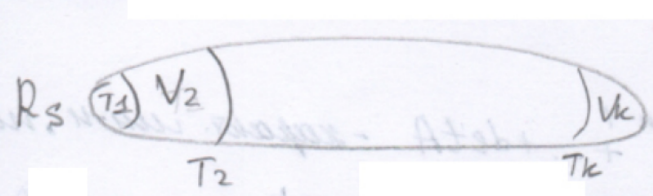
\includegraphics[width=0.5\linewidth]{"images/Issue7-1.png"}
  \caption[]{}
\end{figure}

\begin{theorem}
  Пусть $i > j$, тогда $\forall \vec{h}_i \in \mathcal{V}^i \, \exists \vec{h}_j \in \mathcal{V}^j: \vec{h}_j = B^{i-j}\vec{h}_i$.
\end{theorem}

\begin{proof}
  Построим такой $\vec{h}_j$ и покажем, что он лежит в $\mathcal{V}^j$.

  \[ B^j \vec{h}_j = B^j (B^{i-j}(h_i)) = (B^j B^{i-j} )(\vec{h}_i) = B^i \vec{h}_i = 0 \] 
  \[ B^{j-1} \vec{h}_j = B^{j-1} (B^{i-j}(h_i)) = (B^{j-1} B^{i-j} )(\vec{h}_i) = B^{i-1} \vec{h}_i \neq 0 \]
\end{proof}

Построение соответствующего базиса начинается с определения собственных векторов $A$, соответствующих числу $\bar{\lambda}$.
Для этого решается уравнение $(\bar{A} - \bar{\lambda} E) \vec{\bar{x}} = B  \vec{\bar{x}} = 0$.

Рассмотрим случай, когда имеется только один собственный вектор $\vec{e}$. В этом случае $k = l$ (наше подпространство будет представимо в виде 1 жордановой клетки). 
Вектор $\vec{e}$ образует базис в $\mathcal{V} = T_1$. Вектор $\vec{h}_1 \in \mathcal{V}^2$ найдём как решение $B \vec{h}_1 = \vec{e}$, по доказанной выше теореме такое уравнение имеет решение. 
Вектор $\vec{h}_1$ называется \textbf{присоединенным} к вектору $\vec{e}$. Вектора $\vec{e}$ и $\vec{h}_1$ образуют базис в $T_2$. 
Определим векторы $\vec{h}_i$, $i = \overline{2, l-1}$ из уравнений $B \vec{h_i} = \vec{h}_{i-1}$. Так построенные векторы $\vec{e}, \vec{h}_1, ..., \vec{h}_{l-1}$ образует базис в $R_s$. 
Этот базис называется жордановой цепью.

Запишем матрицу системы в этом базисе. Все построенные векторы находим из уравнений: 
$\bar{A}\vec{e} = \bar{\lambda} \vec{e}$, $\bar{A} \vec{h}_1 = \vec{e} + \bar{\lambda} \vec{h}_1$, ..., $\vec{A} \vec{h}_{l-1} = \vec{h}_{l-2} + \bar{\lambda} \vec{h}_{l-1}$

\[ \bar{A} = \begin{Vmatrix*} \bar{\lambda} & 1 & 0 & \cdots & \cdots \\
                              0 & \bar{\lambda} & 1 & 0 & \cdots     \\
                              \cdots & \cdots & \ddots & \cdots & \cdots \\
                              \cdots & \cdots & \cdots & \bar{\lambda} & 1 \\ 
                              \cdots & \cdots & \cdots & 0 & \bar{\lambda} 
             \end{Vmatrix*} \text{ - жорданова клетка размер $l$}
             \]

В таком базисе системе имеет вид:

\begin{equation}
 \begin{cases}
   \cfrac{d \bar{x}^{\,1}}{dt} = \bar{\lambda} \bar{x}^{\,1} + \bar{x}^{\,2} \\
   \ldots \\
   \cfrac{d \bar{x}^{\,n-1}}{dt} = \bar{\lambda} \bar{x}^{\,n-1} + \bar{x}^{\,n} \\
   \cfrac{d \bar{x}^{\,n}}{dt} = \bar{\lambda} \bar{x}^{\,n} \\
 \end{cases} 
\end{equation}

Замена: $\bar{x}^{\,i} = \bar{y}^{\,i} e^{\bar{\lambda} t}$, $i = \overline{1, l} \Rightarrow \dot{\vec{y}}^{\,i} e^{\bar{\lambda} t} + \bar{\lambda} \dot{\vec{y}}^{\,i} e^{\bar{\lambda} t} = \lambda \dot{\vec{y}}^{\,i} e^{\bar{\lambda} t} + \dot{\vec{y}}^{\,i+1} e^{\bar{\lambda} t} \Rightarrow$
Система преобразуется к виду:

\begin{equation}
  \begin{cases}
    \cfrac{d\bar{y}^{\,1}}{dt} = \bar{y}^{\,2} \\ 
    \cfrac{d\bar{y}^{\,2}}{dt} = \bar{y}^{\,3} \\
    \ldots \\
    \cfrac{d\bar{y}^{\,l-1}}{dt} = \bar{y}^{\,l} \\
    \cfrac{d\bar{y}^{\,l}}{dt} = 0
  \end{cases}
  \Rightarrow 
  \vec{y} = \begin{Vmatrix*} c_l \cfrac{t^{l-1}}{(l-1)!} + c_{l-1} \cfrac{t^{l-2}}{(l-2)!} + ... + c_2 \cfrac{t}{1!} + c_1 \\
                            \ldots \\
                            \ldots \\
                            c_l t + c_{l-1} \\
                            c_l \end{Vmatrix*} \Rightarrow  
\end{equation}

\begin{equation*}
  \Rightarrow \vec{\bar{x}} = \begin{Vmatrix*} c_l \cfrac{t^{l-1}}{(l-1)!} + c_{l-1} \cfrac{t^{l-2}}{(l-2)!} + ... + c_2 \cfrac{t}{1!} + c_1 \\
    \ldots \\
    \ldots \\
    c_l t + c_{l-1} \\
    c_l \end{Vmatrix*} \cdot e^{\bar{\lambda} t} 
\end{equation*}


Переходим к старому базису: 

\[ \vec{x}(t) = \begin{Vmatrix*}
  \vec{e}, \vec{h}_1, ..., \vec{h}_{l-1} 
\end{Vmatrix*} \cdot \begin{Vmatrix*} c_l \cfrac{t^{l-1}}{(l-1)!} + c_{l-1} \cfrac{t^{l-2}}{(l-2)!} + ... + c_2 \cfrac{t}{1!} + c_1 \\
\ldots \\
\ldots \\
c_l t + c_{l-1} \\
c_l \end{Vmatrix*} \cdot e^{\bar{\lambda} t} \Rightarrow \] 

\begin{multline}
 \vec{x}^{\text{ об}}_0 =  \vec{e} \left(c_1 + ... + c_l \cfrac{t^{l-1}}{(l-1)!} \right) e^{\bar{\lambda} t} + ... + \vec{h}_{l-1} c_l e^{\bar{\lambda} t} = \\ 
  = \boxed{c_1 \vec{e} e^{\bar{\lambda} t} + c_2 (\vec{e} t + \vec{h}_1) e^{\bar{\lambda} t} + ... + c_l \left[ \vec{e} \cfrac{t^{l-1}}{(l-1)!} + \vec{h}_1 \cfrac{t^{l-2}}{(l-2)!} + ... + \vec{h}_{l-1} \right]} 
\end{multline}

Полагая последовательно $c_1 = 1, c_2 = ... = c_n = 0$; ...; $c_1 = ... = c_{i-1} = c_{i+1} = ... = c_n = 0$, $c_i = 1$, $i = \overline{2, n}$ получим функции:

$\vec{\varphi}_1 = \vec{e} e^{\bar{\lambda} t}$, $\vec{\varphi}_1 = (\vec{e}t + \vec{h}_1) e^{\bar{\lambda} t}$, ..., $\vec{\varphi}_{l-1} = \left(\vec{e} \cfrac{t^{l-1}}{(l-1)!} + \vec{h}_1 \cfrac{t^{l-2}}{(l-2)!} + ... + \vec{h}_{l-1}\right) e^{\bar{\lambda} t}$. 
Они являются решениями по построению, $W(0) = \begin{vmatrix*} ||\vec{e}, ..., \vec{h}_{l-1} ||\end{vmatrix*} \neq 0 \Rightarrow \vec{\varphi}_1, ..., \vec{\varphi}_{l-1}$ -- линейно независимы $\Rightarrow \vec{\varphi}_1, ..., \vec{\varphi}_{l-1}$ -- ФСР. 

\subsection{Линейная неоднородная система уравнений в случае, когда неоднородность представлена векторным квазимногочленом (без доказательства)}

\textbf{Источник: Романко В.К. Курс дифференциальных уравнений и вариационного исчисления}

\begin{definition}
  \textbf{Вектор-квазимногочленом} называется вектор-функция $f(t) = e^{\mu t} P_m(t)$, где $\mu$ -- заданное комплексное число, $P_m(t)$ -- вектор-многочлен степени $m$, коэффициентами которого служат $n$-мерные векторы. 
\end{definition}

\begin{theorem}
  Если в системе $\dot{x}(t) = A x(t) + f(t)$ $f(t) = e^{\mu t} P_m(t)$, где $P_m(t)$ -- вектор-многочлен степени $m$, тогда для этой системы всегда существует решение вида
  \[ x(t) = e^{\mu t} Q_{m+k}(t)\]
  где $Q_{m + k}$ -- вектор-многочлен степени $(m + k)$, причём $k = 0$, если $\mu$ -- не собственное значение $A$, и $k$ не превосходит наибольшей длины жордановой цепочки для $\mu$, если $\mu$ -- собственное значние $A$, а коэффициентами $Q_{m+k}(t)$ служат $n$-мерные числовые вектора.
\end{theorem}
    \subsection{Формула Лиувилля-Остроградского для нормальной линейной однородной системы уравнений и для линейного однородного уравнения n-го порядка.}

Следующее свойство вронскиана рассмотрим в виде теоремы. Для начала докажем вспомогательное утверждение.

\begin{lemma}

[Формула Эйлера дифференцирования определителя]\\
Детерминант матрицы представим в виде: 
$\Delta = 
\begin{vmatrix}
  a_1^1 & ... & a_n^1 \\
  a_1^i & ... & a_n^i \\
  ...   & ... & ...   \\
  a_1^n & ... & a_n^n \\
\end{vmatrix} = \sum\limits_{k = 1}^n{(-1)^{k + i} \cdot {a_k}^i {M_i}^k}
$
Тогда для 
\[\dot{\Delta}(t) = \sum\limits_{i = 1}^n{\sum\limits_{j = 1}^n{(-1)^{i + j} \cdot \dot{a_j^i}}M_i^j}\]

\end{lemma}

\begin{theorem}

[Формула Лиувилля-Остроградского]\\
Пусть $W(x) - $ вронскиан решений $\vec{\varphi_1}(t), ..., \vec{\varphi_n}(t)$ однородной системы $\dot{\vec{x}} = A\vec{x}$. Тогда имеет место формула:

\[\dot{W(t)} = W(t) \cdot trA\]
где $trA = \sum\limits_{k = 1}^n{a_{kk}(t)}$

\end{theorem}

\begin{proof}

Зафиксируем среди системы решений функцию $\vec{\varphi_j}=
\begin{pmatrix}
  \varphi_j^1 \\
  \varphi_j^2 \\
  ...   \\
  \varphi_j^n \\
\end{pmatrix}
$.
Рассмотрим i - ую компоненту $\varphi_j^i$ решения $\vec{\varphi_j}$. Поскольку $\vec{\varphi_j}$ решение, то $\frac{d\vec{\varphi_j}}{dt} = A\vec{\varphi_j} \Rightarrow$

\[\frac{d\varphi_j^i}{dt} = \dot{\varphi_j^i} = \sum\limits_{k = 1}^n{a_k^i \varphi_j^k}\]

Рассмотрим вранскиан $W(t)$, продифференцируем его по $t$

\[\dot{W}(t) = \sum\limits_{i = 1}^n{\sum\limits_{j = 1}^n{(-1)^{i + j} \cdot \dot{\varphi_j^i} M_j^i}} = \sum\limits_{i = 1}^n{\sum\limits_{j = 1}^n{\sum\limits_{k = 1}^n{(-1)^{i + j} \cdot a_k^i \varphi_j^k M_j^i}}}\]

Переставим суммы местами

\[\dot{W}(t) = \sum\limits_{k = 1}^n{\sum\limits_{i = 1}^n{a_k^i}{\sum\limits_{j = 1}^n{(-1)^{i + j} \varphi_j^k M_j^i}}} = \sum\limits_{k = 1}^n{\sum\limits_{i = 1}^n{a_k^i}\delta_i^k W(t)} = W(t)\sum\limits_{k = 1}^n{\sum\limits_{i = 1}^n{a_k^i}\delta_i^k} = W(t)\sum\limits_{k = 1}^n{a_k^k}\]

\[\dot{W}(t) = W(t) \cdot trA\]

\end{proof}

Также можно решить это уравнение и переписать в виде

\[W(t) = W(t_0)\exp{\left(\int\limits_{t_0}^{t}trA(u)du\right)}\]

\subsection{Метод вариации постоянных для линейной неоднородной системы уравнений и для линейного неоднородного уравнения n-го порядка.}

\begin{equation}\label{eq10_1}
\text{Рассмотрим} ~ y^{(n)} + a_1(x)y^{(n-1)} + ... + a_n(x)y = f(x).\\
\end{equation}

$\varphi_1(x),~...,~\varphi_n(x)$ -- Ф.С.Р. однородного уравнения $y^{(n)} + a_1(x)y^{(n-1)} + ... + a_n(x)y = 0$. Это означает, что 

\begin{equation}\label{eq10_2}
\forall k = \overline{1,n} \hookrightarrow \varphi_k^{(n)} + a_1(x)\varphi_k^{(n-1)} + ... + a_n(x)\varphi_k \equiv 0
\end{equation}

Перепишем уравнение $(\ref{eq10_1})$ в эквивалентном виде. Для этого сделаем следующие замены: $y = v_1, ~y^{(1)} = v_2,~..., ~y^{(n-1)} = v_n$. Тогда получим:

\begin{equation}\label{eq10_3}
 \begin{cases}
   \frac{dv_1}{dx} = v_2, 
   \\
   \frac{dv_2}{dx} = v_3,
   \\
   ...,
   \\
   \frac{dv_n}{dx} = f(x) - a_1(x)v_n - ... - a_n(x)v_1.
 \end{cases}
\end{equation}

Будем искать решение $(\ref{eq10_1})$ в виде
\[y(x) = C_1(x)\varphi_1(x) + ... + C_n(x)\varphi_n(x)\]

Тогда получается, что решение эквивалентной системы будем искать в виде

\begin{equation}
\vec{v}(x) = 
	\begin{Vmatrix}
  		v_1(x)\\
  		...\\
  		v_n(x)
	\end{Vmatrix} = C_1(x)
		\begin{Vmatrix}
  			\varphi_1(x)\\
  			...\\
  			\varphi_1^{(n-1)}(x)
		\end{Vmatrix} + ... + C_n(x)
			\begin{Vmatrix}
  				\varphi_n(x)\\
  				...\\
  				\varphi_n^{(n-1)}(x)
			\end{Vmatrix}
\end{equation}

Рассмотрим функцию $v_k(x) = C_1(x)\varphi_1^{(k-1)} + ... + C_n(x)\varphi_n^{(k-1)}$. Продифференцируем эту функицю по $x$:
\begin{equation}
\forall k =\overline{1, n-1} \hookrightarrow \dot{v_k}(x) = \dot{C_1}(x)\varphi_1^{(k-1)} + ... + \dot{C_n}(x)\varphi_n^{(k-1)} + C_1(x)\varphi_1^{(k)} + ... + C_n(x)\varphi_n^{(k)}
\end{equation}

С другой стороны $\dot{v_k}(x) = v_{k+1} = C_1(x)\varphi_1^{(k)} + ... + C_n(x)\varphi_n^{(k)}$. Тогда получаем
\begin{equation}
\dot{v_k}(x) = C_1(x)\varphi_1^{(k)} + ... + C_n(x)\varphi_n^{(k)} = \dot{C_1}(x)\varphi_1^{(k-1)} + ... + \dot{C_n}(x)\varphi_n^{(k-1)} + C_1(x)\varphi_1^{(k)} + ... + C_n(x)\varphi_n^{(k)}
\end{equation}
\begin{equation}
\forall k =\overline{1, n-1} \hookrightarrow \dot{C_1}(x)\varphi_1^{(k-1)} + ... + \dot{C_n}(x)\varphi_n^{(k-1)} = 0
\end{equation}
\begin{eqnarray*}
k = n: ~\dot{v_n}(x) = \dot{C_1}(x)\varphi_1^{(n-1)} + ... + \dot{C_n}(x)\varphi_n^{(n-1)} + C_1(x)\varphi_1^{(n)} + ... + C_n(x)\varphi_n^{(n)} = \\ = f(x) - a_1(x)\left(C_1(x)\varphi_1^{(n-1)} + ... + C_n(x)\varphi_n^{(n-1)}\right) - ... - a_n(x)\left(C_1(x)\varphi_1 + ... + C_n(x)\varphi_n\right)
\end{eqnarray*}

\begin{eqnarray*}
\dot{C_1}(x)\varphi_1^{(n-1)} + ... + \dot{C_n}(x)\varphi_n^{(n-1)} + C_1(x)\left(\varphi_1^{(n)} + a_1(x)\varphi_1^{(n-1)} + ... + a_n(x)\varphi_1\right) + ... + \\ + C_n(x)\left(\varphi_n^{(n)} + a_1(x)\varphi_n^{(n-1)} + ... + a_n(x)\varphi_n\right) = f(x)
\end{eqnarray*}

Из уравнения $(\ref{eq10_2})$ следует что выражения в скобках равны нулю, тогда получим

\[k = n: ~\dot{C_1}(x)\varphi_1^{(n-1)} + ... + \dot{C_n}(x)\varphi_n^{(n-1)} = f(x)\]

Т.е. мы получили следующую систему уравнений:
\begin{equation}\label{eq10_4}
 \begin{cases}
   \dot{C_1}(x)\varphi_1 + ... + \dot{C_n}(x)\varphi_n = 0, 
   \\
   ...
   \\
   \dot{C_1}(x)\varphi_1^{(n-2)} + ... + \dot{C_n}(x)\varphi_n^{(n-2)} = 0,
   \\
   \dot{C_1}(x)\varphi_1^{(n-1)} + ... + \dot{C_n}(x)\varphi_n^{(n-1)} = f(x).
 \end{cases}
\end{equation}
Система $(\ref{eq10_4})$ это линейная система для определения $\dot{C_1}, ~..., ~\dot{C_n}$.
Определитель этой системы $\Delta = W(x) \neq 0$, а значит система разрешима единственным образом.
    \subsection{Теорема Штурма}

Рассмотрим на промежутке $I = I(x)$ следующее уравнение:

\begin{equation}\label{diff-eq_issue12}
y'' + a(x)y' + b(x)y = 0,
\end{equation}

где $a(x) \in C^1_{I(x)}$, $b(x) \in C^1_{I(x)}$.

Решение (\ref{diff-eq_issue12}) такое, что $y(x)$ тождественно не равно нулю на $I(x)$ называется нетривиальным , а точка $x_0 \in I$ такая, что $y(x_0) = 0$ называется нулём нетривиального решения $y(x)$.

Уравнение (\ref{diff-eq_issue12}) приводится к виду:

\begin{equation}\label{diff-eq_z-form_issue12}
z'' + q(x)z = 0.
\end{equation}

Для этого сделаем замену $y(x) = c(x) \cdot z(x)$, где $z(x)$ - решение уравнения выше (далее будем считать, что $c = c(x)$ и $z = z(x)$:

\[z''\cdot c + 2c' \cdot z' + c'' \cdot z + a(x) (c' \cdot z + z' \cdot c) + b(x) \cdot c \cdot z = 0,\]

здесь выберем $c \neq 0$ так, что бы для $z'$ выполнялось:

\[z' (2c' + a(x) c) = 0.\]

Тогда получаем линейное однородное уравнение $\Rightarrow \: 2c' + a(x)c = 0$, которое можно преобразовать в:

\begin{equation}\label{c-x-solution_issue12}
\frac{dc}{c} = - \frac{a(x)}{x}dx\: \Rightarrow \: c(x) = c_0 \cdot exp \left[-\frac{1}{2} \int a(x)dx\right] > 0.
\end{equation}

Возьмем $c_0 = 1 \: \Rightarrow \: c \cdot z'' + (c'' + c'a + bc)z = 0$, тогда можемм ввести $q(x)$ такое, что:

\[q(x) = \frac{c'' + c'a}{c} + b.\]

Также заметим, что из (\ref{c-x-solution_issue12}) следует, что $c(x) > 0$. Тогда в силу замены $y = c(x) \cdot z$, $x_0 \in I$ является нулём $y(x)$ тогда и только тогда, когда $x_0$ является нулём $z(x)$.

\begin{definition}
Точка $x_0$ является нулём $f(x) \in C^{\infty}$ кратности $k$, если $f(x_0) = f'(x_0) = ... = f^{(k-1)}(x_0) = 0$, а $f^{(k)}(x_0) \neq 0$.
\end{definition}

\begin{lemma}\label{sol-zeros_issue12}
Все нули нетривиального решения (\ref{diff-eq_z-form_issue12}) (также как и для (\ref{diff-eq_issue12})) являются простыми, т.е. $k = 1$.
\end{lemma}

\begin{proof}
От противного: пусть $x_0$ является нулём кратности 2, тогда $z(x_0) = z'(x_0) = 0$. Тогда в силу основной теоремы $z(x) = 0 \forall x \in I$ - противоречие, т.к. $z(x)$ - нетривиальное решение по условию.
\end{proof}

\begin{lemma}\label{sol-set_issue12}
Пусть M - множество нулей нетривиального решения $y(x)$ на нечетном промежутке $[x_1;x_2]$. Множество M не имеет предельной точки.
\end{lemma}

\begin{proof}
От противного: пусть M - множество нулей. Пусть $x_0$ - предельная точка и $\exists {x_k} :$ 

\[\deflimk x_k = x_0 \in [x_1;x_2], \: y(x_k) = 0, \: k = 1,2,...\]

Так как $y(x)$ - непрерывно, то $\deflimk y(x_k) = 0 = y (\deflimk x_k) = y(x_0) \: \Rightarrow \: y(x_0) = 0$.

Рассмотрим $[x_k;x_{k+1}]$ и $y(x)$ на нём, т.к. $y(x_k) = y(x_{k+1}) = 0$, то по теореме Ролля $\exists c_k: x_k \leq c_k \leq x_{k+1}: y'(c_k) = 0$ и т.к. $\deflimk x_k = \deflimk x_{k+1} = x_0 \Rightarrow \deflimk c_k = x_0$. Из этого может получить, что так как $y'(x)$ - непрерывна, то:

\[\deflimk y' (c_k) = 0 = y' (\deflimk c_k) = y'(x_0) = 0\]

Так как по предложению $x_0 \in [x_1;x_2]$ и $y_0(x_0) = 0$, $y'(x_0) = 0$ - получим задачу Коши для $x_0 \in [x_1;x_2] \Rightarrow$ в силу теорем существования и единственности решения задачи Коши: $y\equiv 0$ - единственное решение на $[x_1;x_2]$ - получим противоречие с нетривиальным решением.
\end{proof}

\begin{theorem}
[Теорема Штурма]

Рассмотрим уравнения:

\begin{equation}\label{fast-eq_issue12}
y'' + q(x) y = 0
\end{equation}

\begin{equation}\label{slow-eq_issue12}
z'' + Q(x)z = 0,
\end{equation}

где уравнение (\ref{fast-eq_issue12}) будем называть быстрым, а (\ref{slow-eq_issue12}) - медленным.

Пусть 

\[q(x)\in C^1_{I(x)}, Q(x) \in C^1_{I(x)}, \forall x \in I \rightarrow q(x) \leq Q(x).\]

Пусть $y(x)$ - нетривиальное решение (\ref{fast-eq_issue12}), z(x) - нетривиальное решение (\ref{slow-eq_issue12}). Если $x_1, x_2 \in I$ - последовательное нули $y(x)$б то либо $\exists x_0 \in (x_1;x_2)$, в которой $z(x_0) = 0$, либо $z(x_1) = z(x_2) = 0$.
\end{theorem}

\begin{proof}
Пусть $x_1, x_2$ - два соседних нуля $y(x)$, т.е. $y(x) \neq 0$ на $(x_1;x_2)$, пусть для определённости $y(x) > 0$.

По определению:

\[y'(x_1) = \lim\limits_{x\rightarrow x_1} \frac{y(x) - y(x_1)}{x - x_1} \geq 0; \: y'(x_2) = \lim\limits_{x\rightarrow x_2} \frac{y(x) - y(x_2)}{x - x_2}.\]

В силу Леммы \ref{sol-zeros_issue12} нули $x_1$ и $x_2$ должны быть однократными, т.е. $y'(x_1) \neq 0, \: y'(x_2) \neq 0$. Таким образом $y'(x_1) > 0, \: y'(x_2) < 0$.

Умножим (\ref{slow-eq_issue12}) на $z(x)$, а (\ref{fast-eq_issue12}) на y(x) и вычтем из первого второе:

\[zy'' + qyz - yz''' - Qyz = 0; \: zy'' - yz'' = (zy'-yz')' = (Q - q)zy.\]

Проинтегрируем полученное тождество на $[x_1;x_2]$:

\[(zy' - yz')\Big\vert_{x_1}^{x_2} = \int\limits_{x_1}^{x_2} (Q(x) - q(x))zydx;\]

\[z(x_2)y'(x_2) - y(x_2)z'(x_2) - z(x_!)y'(x_1) + y(x_1)z'(x_1) = \int\limits_{x_1}^{x_2}(Q(x) - q(x))zydx \Rightarrow\]

\begin{equation}\label{add-diff_issue12} % additional differential equation
\Rightarrow z(x_2)y'(x_2) - z(x_1)y'(x_1) = \int\limits_{x_1}^{x_2}(Q(x) - q(x))zydx,
\end{equation}

здесь $z(x_2)y'(x_2) < 0$, $z(x_1)y'(x_1) > 0$, $(Q(x) - q(x)) > 0$ и $y > 0$.

Предположим противное - пусть теорема Штурма не верна. Тогда возможны варианты:

\begin{enumerate}
\item $z > 0 \forall x \in [x_1;x_2].$ Тогда левая часть (\ref{add-diff_issue12}) отрицательна, а правая положительна - противоречие.

\item $z > 0 \forall x \in [x_1;x_2), \: z(x_2) = 0$ - аналогично.

\item $z > 0 \forall x \in (x_1;x_2]б \: z(x_1) = 0$ - аналогично.
\end{enumerate}

Таким образом $\exists x_0 \in (x_1;x_2): \: z(x_0) = 0$. Если $z(x_1) = z(x_2)$, то может быть, что $Q(x) \equiv q(x) \Rightarrow z(x) = const \cdot y(x)$, либо:

\[\exists x* \in (x_1;x_2): \: Q(x*) > q(x*),\]

в силу непрерывности $Q(x)$ и $q(x) \exists \bigtriangleup:$

\[\int\limits_{x* -\bigtriangleup}^{x* + \bigtriangleup} (Q(x) - q(x))z(x)y(x)dx = 0,\]

значит $\exists x_0$, где $z(x)$ меняет знак $\Rightarrow z(x_0) = 0$
\end{proof}

\subsection{Следствия из теоремы Штурма}

\begin{corollary}\label{zero-quant_in-diff_issue12}
Пусть есть уравнение:

\[y'' + q(x)y = 0; \: q(x) \leq0 \forall x \in I(x),\]

тогда любое нетривиальное решение (\ref{slow-eq_issue12}) на $I$ имеет не более одного нуля.
\end{corollary}

\begin{proof}
В качестве второго уравнения можно взять $z'' + Q(x)z = 0$, здесь Q(x) = 0. Пусть решение уравнения (\ref{slow-eq_issue12}) имеет нули $x_1$ и $x_2$ $Q(x) \geq q(x) \Rightarrow 0 \geq q(x)$. Тогда по теореме Штурма любое решение (\ref{fast-eq_issue12}) должно иметь ноль на $(x_1;x_2)$. В качестве решения можем вщять $z\equiv 1$, которое не и имеет нулей $\Rightarrow$ противоречие $\Rightarrow$ для решения (\ref{slow-eq_issue12}) не может быть больше одного нуля.
\end{proof}

\begin{corollary}\label{line-indep-sol-zeros_issue12}
Пусть $\varphi (x)$ и $\psi (x)$ - два линейно независимых нетривиальных решения (\ref{slow-eq_issue12}), $x_1, x_2 \in I$ - два соседних нуля $\varphi (x)$, тогда $\psi (x)$ имеет только один нуль на $(x_1;x_2)$.
\end{corollary}

\begin{proof}
Применим теорему Штурма к двум одинаковым уравнениям $(Q(x) \leq Q(x))$. По теореме Штурма $\psi (x)$ на $(x_1;x_2)$ имеет хотя бы один нуль. Общих нулей $\varphi (x)$ и $\psi (x)$ иметь не могут, так как они линейно независимые ($W(x_1) = 0$, если бы $\varphi (x_1) = \psi (x_1) = 0$, что означало бы, что $\varphi(x)$ и $\psi(x)$ - ЛЗ). Итак, $\psi (x)$ имеет нуль $x_0$ на $(x_1;x_2)$.

Докажем, что такой нуль единственный - от противного: пусть нулей два для $\psi (x): x*$ и $\overline{x}$. Если нулей $\psi (x)$ два, то по теореме Штурма для $\varphi (x)$ будет ноль между $x*$ и $\overline{x}$ - противоречие тому, что $x_1$ и $x_2$ соседние нули $\varphi (x)$.
\end{proof}

Таким образом нули решений (\ref{diff-eq_issue12}) перемешаются.
\end{document}